%\documentclass{article}
\documentclass[prl, longbibliography]{revtex4-2}
\usepackage{graphicx}
\usepackage{makecell}
\usepackage{amsmath}
\usepackage{fontspec}
\usepackage{bbold}
%\usepackage{mathtools}
%\usepackage{mathrsfs}
\begin{document}

\title{Mark's Notes on Molecular Potential Calculations, test!}
\author{Mark O. Brown}
\date{\today}

\begin{abstract}
These notes describe the calculation of very long range S+P molecular potentials, including the leading order Born-Oppenheimer (BO) potentials ($1/r^3$ dipole interactions for Homonuclear S+P), fine structure, and hyperfine structre. 
The BO potentials are diagonal in the standard Hund's "case A" molecular basis, and the fine and hyperfine structure are diagonal in the separate atom "F" angular momentum basis. 
The procedure consists of constructing the hamiltonians for each of these energies in a properly single symmetrized  basis and diagonalizing the result as a function of internuclear distance.
While it is trivial to state the procedure, identifying and keeping track of the symmetries in these calculations is rather nuanced and not clearly discussed in the literature. 
These notes therefore aim to discuss this procedure in a very pedagocial manner so that it is easy to repeat these or similar calculations without prior experience in such calculations. 
\end{abstract}

\maketitle

\section{Introduction}

Recent experiments \cite{brown_gray-molasses_2019} involving ultracold atoms in optical tweezers utilize the physics of very long-range molecular interactions in regimes previously not accessible to experiment. 
The experiments typically use molecular collisions in order to selectively heat pairs of atoms out of optical dipole traps on the order of 10MHz deep. 
As such, these experiments are sensitive to the molecular structure of these molecules on the order of 10MHz. While there exists a great deal of literature on the structure of molecular potentials \cite{jones_ultracold_2006}, At these long ranges, the hyperfine interactions are important and measurable, however very few calculations of molecular potentials including the hyperfine interactions exist. 
One such example is \cite{kemmann_near-threshold_2004}, however no discussion of the methods used to calculate the potentials given was ever published. 
In this work, we endeavor to pedagogically discuss how to calculate the molecular potentials, including long-range interactions, for any homonuclear alkali molecule, although the work should be easily extended to different types of atoms. 
In this paper we discuss the theory of the calculation, and available online is an easily accessible Jupyter notebook containing the calculation in the python language.

The problem is simply stated: we must diagonalize $H=H_{BO}+H_{FS}+H_{HFS}$ as a function of distance. However, there are a number of subtleties involved in constructing the hamiltonians in the appropriate well-symmetrized base. This is the majority of the problem. 

\section{Symmetries and quantum numbers}

\subsection{Introduction}
The symmetries of the problem are very important on a number of levels. 
In the first place, the full hamiltonian for Rb87 would be 384x384 in size, but represented in the right basis it is block-diagonal in much smaller chunks, and is therefore numerically much easier to manage. 
In addition, identifying the symmetries of the states helps to build intuition and identify patterns in the resulting molecular potentials, which have a tendency to look like spaghetti otherwise. 
Lastly, the symmetries of the state are important for identifying selection rules for the excitation of these states.

In the end, we will consider 15 different angular momentum operators and their projections on either an arbitrary axis (the "space-fixed" axis) or the molecular axis (the "body-fixed" axis).  
Not only that, but many of the labels of these angular momentum follow arcane rules established in early spectroscopy experiments. 
It's therefore important that the notation here is clear and each angular momentum and projection is clearly identified. 
I will always refer to operator symbols with a hat while symbols without a hat are eigenvalues. 
Unless specifically mentioned otherwise, the eigenvalues will have the exact same symbol except without the hat. For example, $\hat{\mathbb{i}}_{e}$ is an inversion operator to be discussed later, and $i_e=\pm 1$ are the eigenvalues of this operator. 

\subsection{Separate-Atom Quantum Numbers and Interactions}
Since we will eventually be discussing two atoms, I will go ahead and add a subscript $\alpha$ which takes values either $1$ or $2$ to indicate which atom the opeartor applies to.
A single atom is spherically symmetric, and the uncoupled quantum numbers that describe it are: the principle quantum number $n_\alpha$, the orbital angular momentum $L_\alpha$, the electron spin angular momentum $S_\alpha$, and the nuclear spin angular momentum $I_\alpha$, and associated projections $m_{L_\alpha}, m_{S_\alpha}, $ and $m_{I_\alpha}$. 
This completely uncoupled basis can therefore be represented in a long ket as $|n_\alpha L_\alpha m_{L_\alpha} S_\alpha m_{S_\alpha} I_\alpha m_{I_\alpha}\rangle$.
The fine structure interaction is $\propto L_\alpha\cdot S_\alpha$ which commutes with $L^2_\alpha$ and $S^2_\alpha$ but not $L_{z\alpha}$ or $S_{z\alpha}$.
As a result, we introduce the new total single-electron angular momentum $J_\alpha=L_\alpha+S_\alpha$, and therefore we introduce the FS-coupled basis $|n_\alpha L_\alpha S_\alpha J_\alpha m_{J\alpha} I_\alpha m_{I_\alpha}\rangle$.
The Hyperfine interaction is roughly $\sim J\cdot I$, encouraging the introduction of a new total single-atom angular momentum $F_\alpha$, and we therefore introduce the HFS-coupled basis $|n_\alpha L_\alpha S_\alpha J_\alpha I_\alpha F_\alpha m_{F_\alpha}\rangle$. 
This is the basis typically used for atomic physics, although depending on the context it is common to omit many of these extraneous uncoupled quantum numbers. 
For example the common label for fine structure manifolds is $^{2S+1}L_J$, where $L$ is replaced by S for $L=0$, P for $L=1$, D for $L=2$, etc.

\subsection{Born-Oppenheimer Interactions and Symmetries}
Introducing a second atom breaks the spherical symmetry of a single atom.
Many of the remaining symmetries are spatial symmetries of the problem respecting various aspects of the cylindrical symmetry of the problem, so for discussions of the coordinates of the particles in the problem we will consider our coordinate system to be such that the center of mass and charge is at the origin, and the intermolecular axis is aligned along the z-axis. 
Thankfully, for homonuclear atoms the center of charge is the same as the center of mass of the molecule, and so we avoid some minor complications which are encountered with heteronuclear molecules.
Therefore, we start here with the symmetries that are valid with BO interactions but without FS or HFS interactions, and will then work to build the FS and HFS interactions back into the problem.

In general, the interactions between the atoms couples states of different $n_\alpha$ and $L_\alpha$, so none of these are good quantum numbers anymore. In addition, the orientation of the molecule is the only axis of symmetry in the problem, and so only the projection of the angular momentum in the problem which is conserved is that along the internuclear axis. 
In general, since $L_\alpha$ aren't good quantum numbers, it only makes sense to consider the total projection of both angular momentum along this axis, which is typically defined as $\Lambda=L_{1z}+L_{2z}$. 
In general, I will follow the pattern that projections along arbitrary axes, for example in the separate atom case above, are represented by $m$ subscripted with the lattin letter corresponding to its angular momentum (e.g. $m_L$), whereas projections that are specifically along the molecular axis will always be represented by greek letters.
Furthermore, similar to the way L is replaced by S, P, D, etc. for single atom labels, $\Lambda$ will be represented as $\Sigma$ if $\Lambda=0$, $\Pi$ if $\Lambda=1$, $\Delta$ if $\Lambda=2$, etc.

The BO interactions are primarily based on the electric interactions of the electrons with each other and the two nuclei, so BO states still have good values of the total electron spin $S=S_1+S_2$, and can be therefore classified by this quantum number.

The long-range interaction can be modeled as a simple dipole-dipole interaction:

$$
V_{dd} = \frac{1}{4\pi\epsilon_0} \frac{\vec{d}_1\cdot\vec{d}_2-3d_{1z'}d_{2z'}}{R^3} \\
=\frac{e^2}{4\pi\epsilon_0} \frac{\hat{r}_1\cdot\hat{r}_2-3z_{1}z_{2}}{R^3} \\
= -pC_3\frac{3\Lambda^2-L(L+1)}{R^3}
$$

where I want to prove the last result. The states can be described in terms of the single-particle basis as
$$
|L=1,\Lambda=\lambda p\rangle= \frac{1}{\sqrt{2}} (|00,1\lambda\rangle+p|1\lambda,00\rangle)
$$

making the dipole interaction
$$
V_{dd} = \frac{e^2}{4\pi\epsilon_0} \frac{\hat{r}_1\cdot\hat{r}_2-3z_{1}z_{2}}{R^3} \\
$$
\subsection{Geometric Symmetries}

Homonuclear molecules belong to the point group $D_{\infty h}$, which provides for an easy baseline to discuss the relevant symmetries here for the mathematically inclined. A good starting point is \cite{hougen_calculation_2001}, and for more discussion see \cite{lefebvre-brion_perturbations_1986}. 

The problem is symmetric under the \emph{inversion} of all of the electronic spatial coordinates. 
I define the inversion operator which does this as $\hat{\mathbb{i}}_e$.
Since swapping these coordinates twice brings us back to the original state, states can either be symmetric or antisymmetric under this inversion. 
Symmetric states are typically referred to as \emph{gerade} (or "g") or \emph{ungerade} ("u") states. 

Finally, the problem is also symmetric under the reflection of the electrons spatial wavefunction across a plane \emph{containing} the internuclear axis, for example the xz plane, which would be equivalent to setting $y_1\rightarrow -y_1$ and $y_2\rightarrow-y_2$ or $\phi\rightarrow -\phi$ where $\phi$ is the polar angle in spherical coordinates.
The operator which does this is typically labeled $\sigma_v$, however since we will have to modify the operator several times as we add fine and hyperfine structure, I represent this operator which only changes the spatial coordinates of the electron as $\hat{\sigma}_{v_L}$ since it doesn't touch the spin. For any state with Quantum numbers $L$ and $\Lambda$, the operation of $\sigma_{v_L}$ is:

$$
\sigma_{v_L}|L\Lambda\rangle = (-1)^{L-\Lambda}|L,-\Lambda\rangle
$$

Similar to the inversion operator, we must have $\sigma _{v_L}=\pm 1$. This symmetry is slightly counterintuitive from an atomic perspective since the normal hydrogen atom wavefunctions are not eigenvalues of this operator. 
This is simply the result of the choice of basis for the functions however, and one can construct good such states easily enough. For example, with an abbreviated uncoupled basis $|n_\alpha L_\alpha m_{L_\alpha}\rangle$, the superpositions $|111\rangle \pm |11,-1\rangle$ are eigenstates of this reflection operator.
Such symmetric states are typically labeled with a $+$ and antisymmetric states with a $-$. While all BO states can be constructed as eigenstates of this operator, if $\Lambda\ne 0$ the states with different reflection parity are degenerate, and this label is sometimes dropped in those circumstances.
It's not too hard to see from the following discussion that there are some ambiguity in the definitions. In particular, in the following I am using the \_\_\_ convention.

There are a number of additional symmetries one can identify for these potentials involving the other uncoupled angular momentum. For example, states that have different projections of the total spin along the internuclear axis (defined as $\Sigma=S_{1z}+S_{2z}$). However, the symmetries already defined are more than enough to identify all the non-degenerate potentials at this level.

Therefore, BO states are typically labeled by four characters representing the values of $2S+1$, $\Lambda$, $\mathbb{i}_{e}$, and $\sigma_{v_L}$ oriented like this $^{2S+1}\Lambda^{\sigma_{v_L}}_{\mathbb{i}_e}$. For example, with $S=1,\Lambda=0,\mathbb{i}_e=1,\sigma_{v_L}=1$, the symbol is $^3\Sigma_g^+$. In addition, even including all values of $\Lambda$ is unnecessary, as states with positive and negative values are degerate, and so typically only the absolute value of Lambda is reported despite it being possible to have negative values of this quantum number.

It is worth noting now, in the far-separated regime we are interested in, the mixing of states with different $L_\alpha$ and $n_\alpha$ is very weak, and the leading order interactions can be modeled as the dipole-dipole interactions between states that do have well defined $L_\alpha$ and $n_\alpha$. So, in the calculations that follow, the bases that are used will have well-defined $L_\alpha$ and $n_\alpha$. 

\subsection{BO with Fine Structure}

The fine structure interaction is
$$
H_{FS} = A_{FS}(L_1\cdot S_1 + L_2 \cdot S_2)
$$

For alkali atoms where there is only one valence electron, S is a spin-1/2 and this interaction can be parameterized by a single constant $A_{FS}$.

Adding the fine structure, similar to the separate atom case, means that $\Lambda$ and $\Sigma$ are no longer good quantum numbers, but that $\Omega=J_{1z}+J_{2z}$ is a good quantum number now. However, similar to the previous case, only the absolute value of $\Omega$ matters. Unlike for $\Lambda$, in the symbols for these states $\Omega$ are just the numeric value of $|\Omega|$. 

In addition, because the fine structure couples states of different $L$ and $S$, the fine-structure interaction inadvertedly also couples states of different values of $\sigma_{v_L}$, making it also not a good quantum number. However, the operator which flips both the spatial component of the the electronic wavefunction \emph{as well as the spin} (effectively flipping both $\hat{L}$ and $\hat{S}$) commutes with the fine structure hamiltonian and will give us good quantum numbers. I will label this slightly different operator $\sigma_{v_{LS}}$. Similarly to the previous case, it is only states with $\Omega=0$ that states with different $\sigma_{v_{LS}}$ are not degenerate.

$$
\sigma_{v_{LS}}|L\Lambda S \Sigma\rangle = (-1)^{L-\Lambda+S-\Sigma}|L,-\Lambda S, -\Sigma\rangle
$$

$i_e$ are still good quantum numbers. Therefore, the symbols for these types of states are of the form $\Omega_{i_e}^{\sigma_{v_{LS}}}$, for example $0_g^+$. The results of adding the fine-structure interactions includes the creation of new deeply bound states which were first predicted by \cite{stwalley_pure_1978}

\subsection{BO with Hyperfine Structure}

The hyperfine fine structure interaction is effectively
$$
H_{HFS} = A_{HFS}(L_1\cdot I_1 + L_2 \cdot I_2)
$$

This can be roughly approximated by a single parameter $A_{HFS}$ but to be accurate at the level required the asymptotic energies must be inputted by hand.

Adding the hyperfine structure follows a similar pattern as with adding the fine structure. In this case, our good projection is now the projection of the total atomic angular momentum defined as $\phi=F_{1z}+F_{2z}$. Similarly, only the absolute value of $\phi$ matters. 

The hyperfine interaction hamiltonian couples states of different $\sigma_{v_{LS}}$, and so we must modify this reflection operator again to have good quantum numbers. Now, if an operator also flips the nuclear spin in addition to the electronic spin and spatial wavefunction, this will commute with our total hamiltonian. Since this is our final reflection operaotr, I will give this one the nice symbol $\sigma_v$. 

$$
\sigma_{v}|L\Lambda S \Sigma I \iota\rangle = (-1)^{L-\Lambda+S-\Sigma+I-\iota}|L,-\Lambda, S, -\Sigma, I, -\iota\rangle
$$

Because we are now considering the nuclear spin, the two nuclear centers are now not necessarily identical, and so now $i_e$ are no longer good quantum numbers. We can construct a similar operator however which inverts both the electrons spatial coordinates as well as the nuclear spatial coordiantes. I will represent this final inversion operator with the nice symbol $\hat{i}$. 

Notation for the labels of these states with molecular potentials is not particularly well established. In the past, Jose and his collaborators have labeled states with $i=1$ as "a" states and states with $i=-1$ as "b" states. As well, they referred to states with $\sigma_v=1$ as "1" states and $\sigma_v=2$ as "2" states. As such, their labels were of the form $\phi i \sigma_v$. I will avoid this convention for these notes (at least for now, perhaps someone will convince me otherwise :)). Since there is such a wealth of confusing notation here, I will opt for a very explicit notation in these notes. States with $i=\pm 1$ will be labeled "$i\pm$", and states with $\sigma_v=\pm1$ will be labeled $\sigma\pm$, in the convenient notation $\phi_i^{\sigma_v}$. The states relevant for Rb87 calculations are then $0_{i+}^{\sigma_v+},0_{i+}^{\sigma_v-},0_{i-}^{\sigma_v-},0_{i+}^{\sigma_v-}, 1_{i+},1_{i-},2_{i+},2_{i-},3_{i+},3_{i-},4_{i+},4_{i-},5_{i+},5_{i-}$. One fairly sensible alternative here is to drop the $i$ and $\sigma_v$ from the labels, and instead label them like $0^+_-$

\begin{center}
\begin{tabular}{ ||c|c|c|c|c|c||  }
 \hline
 Description & \makecell{Angular \\Momentum \\Operator $\hat{Z}$} & \makecell{$\hat{Z}^2$ Eigenvalues \\($\hbar^2 z(z+1)$)} & \makecell{Body-Fixed\\ $\hat{Z}_z$ Eigenvalues \\($\hbar m_z$)} &\makecell{Space-Fixed\\ $\hat{Z}_z$ Eigenvalues \\($\hbar m_z$)} & \makecell{Alternative\\Operator\\Representations}\\
 \hline
 \hline
 Single Electron Orbital A.M. & $\hat{L}_\alpha$ & $L_\alpha$ & $\Lambda_\alpha$ & $m_{L_\alpha} $ & None \\
 \hline
 Total Electron Orbital A.M. & $\hat{L}$ & $l$ & $\Lambda=\Lambda_1+\Lambda_2$ &$m_L $ & $\hat{L}=\hat{L}_1 + \hat{L}_2$ \\
 \hline
 Single Electron Spin & $\hat{S}_\alpha$ & $S_\alpha$ & $\Sigma_\alpha$ &$m_{S_\alpha} $ & None \\
 \hline
 Total Electron Spin & $\hat{S}$ & $S$ & $\Sigma=\Sigma_1+\Sigma_2$ &$m_S $ &  $\hat{S}=\hat{S}_1 + \hat{S}_2$ \\
 \hline
 Single Electron Total A.M. & $\hat{j}_\alpha$ & $j_\alpha$ & $\Omega_\alpha=\Lambda_\alpha+\Sigma_\alpha$ &$m_{j_\alpha} $ &  $j_\alpha = L_\alpha+S_\alpha$ \\
 \hline
 Total Electron A.M. & $\hat{j}$ & $j$ & $\Omega=\Lambda+\Sigma$ &$m_j $  & $\hat{j} = \hat{L}+\hat{S}$ \\
 \hline
% Total A.M. Except Nuclear Spin & $\hat{J}$ & $J$ & Also $\Omega$ &$m_J $  & $\hat{J}=\hat{L}+\hat{S}+\hat{N}$ \\
% \hline
% Nuclear Rotational A.M. & $\hat{N}$ & $\ell$ & $0$ (Always) & $\mu$ &  $\hat{N} = \hat{J} - \hat{L} - \hat{S}$ \\
% \hline
 Single Nuclear Spin & $\hat{i}_\alpha$ & $i_\alpha$ & $\iota_{\alpha}$ &$m_i $ &  None \\
 \hline
 Total Nuclear Spin & $\hat{I}$ & $I$ & $\iota=\iota_1+\iota_2$ &$m_I $ &  $\hat{I}=\hat{i}_1+\hat{i}_2$ \\
% \hline
% \makecell{Total Mechanical A.M.\\(Relevant in Hund's cases (b) and (d))} & $\hat{K}$ & $K$ & (Rare)$\kappa$? &$m_K $ &  $\hat{K}=\hat{L}+\hat{N}$ \\
 \hline
  Single Atom Total A.M. & $\hat{f}_\alpha$ & $f_\alpha$ & $\phi_\alpha=\Omega_\alpha+\iota_{\alpha}$ &  $m_{f_\alpha} $& $\hat{f}_\alpha=\hat{j}_\alpha+\hat{i}_\alpha$ \\
 \hline
   Total Non-Rotatoinal A.M. & $\hat{f}$ & $f$ & $\phi=\Omega+\iota$ &  $m_f $& $\hat{f}=\hat{j}+\hat{i}$ \\
 \hline
%  Total A.M. & $\hat{F}$ & $F$ & Also $\phi$ &$m_F $ &  $\hat{F}=\hat{J}+\hat{I}$ \\
% \hline 
\end{tabular}
\end{center}

\section{Calculation...}

\begin{figure}
  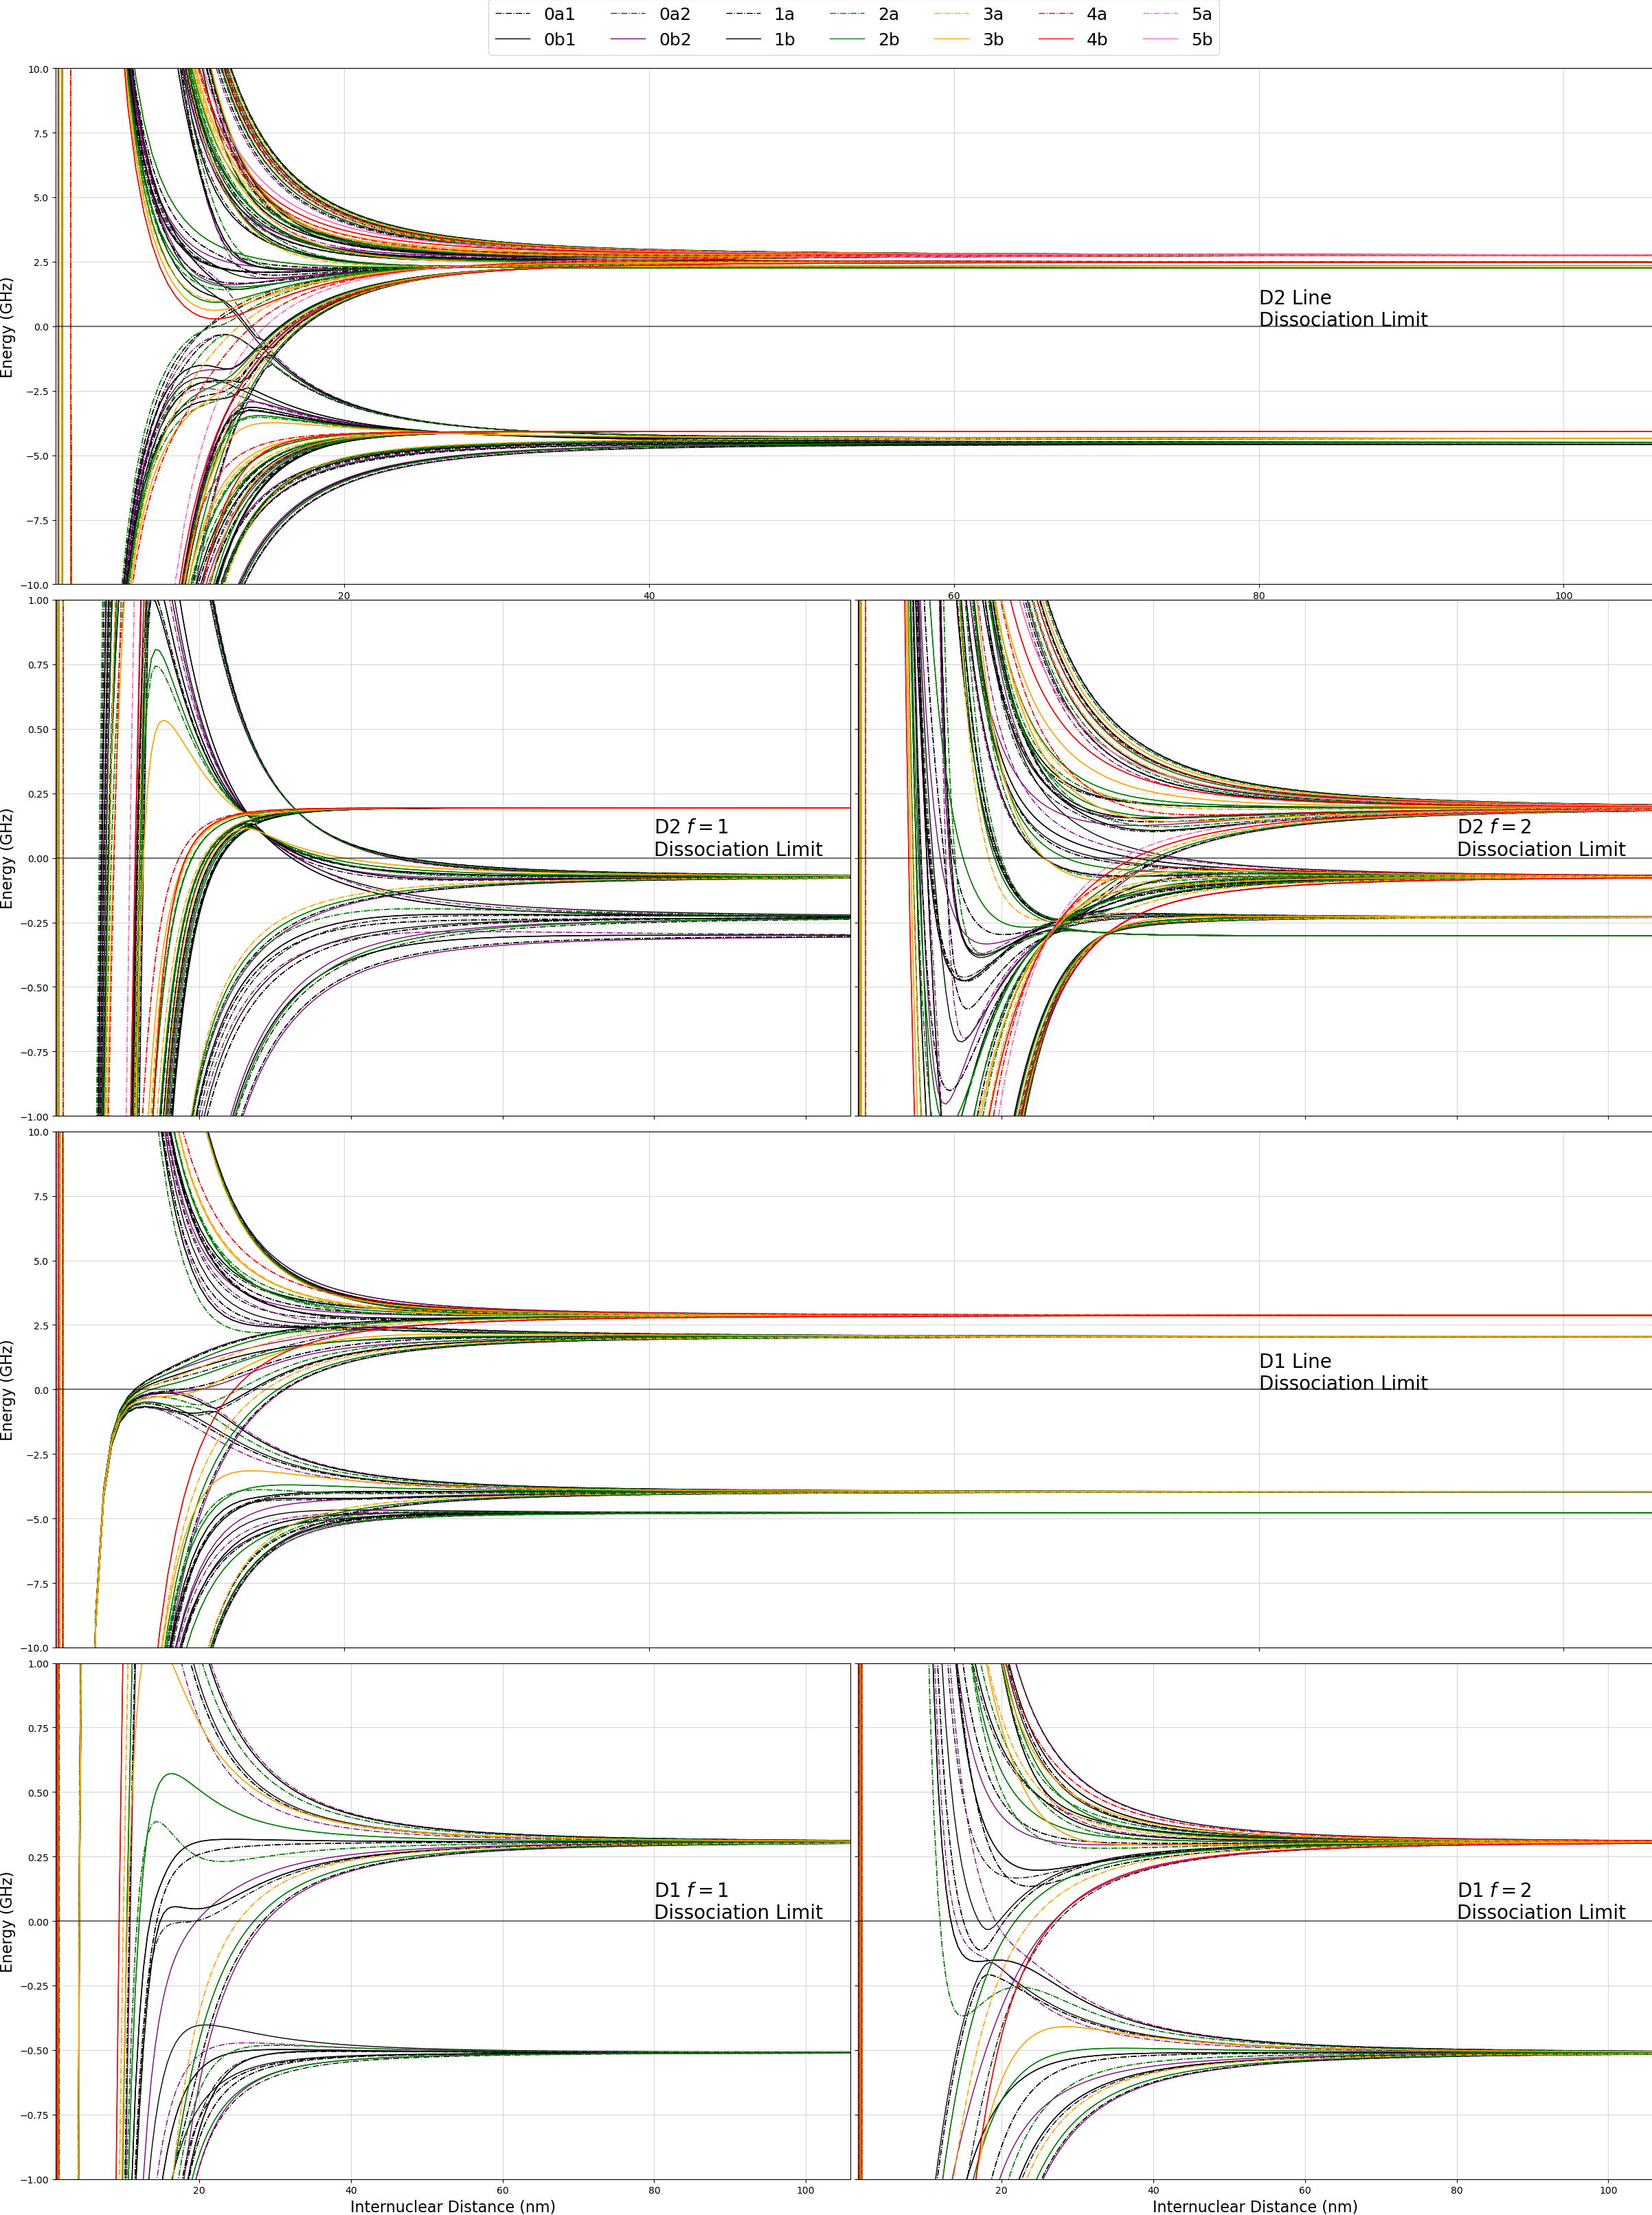
\includegraphics[width=\linewidth]{Symmetrized_Hyperfine_Splitting_Big_Picture.png}
  \caption{A zoomed out view of the potentials.}
  \label{fig:boat1}
\end{figure}
\begin{figure}
  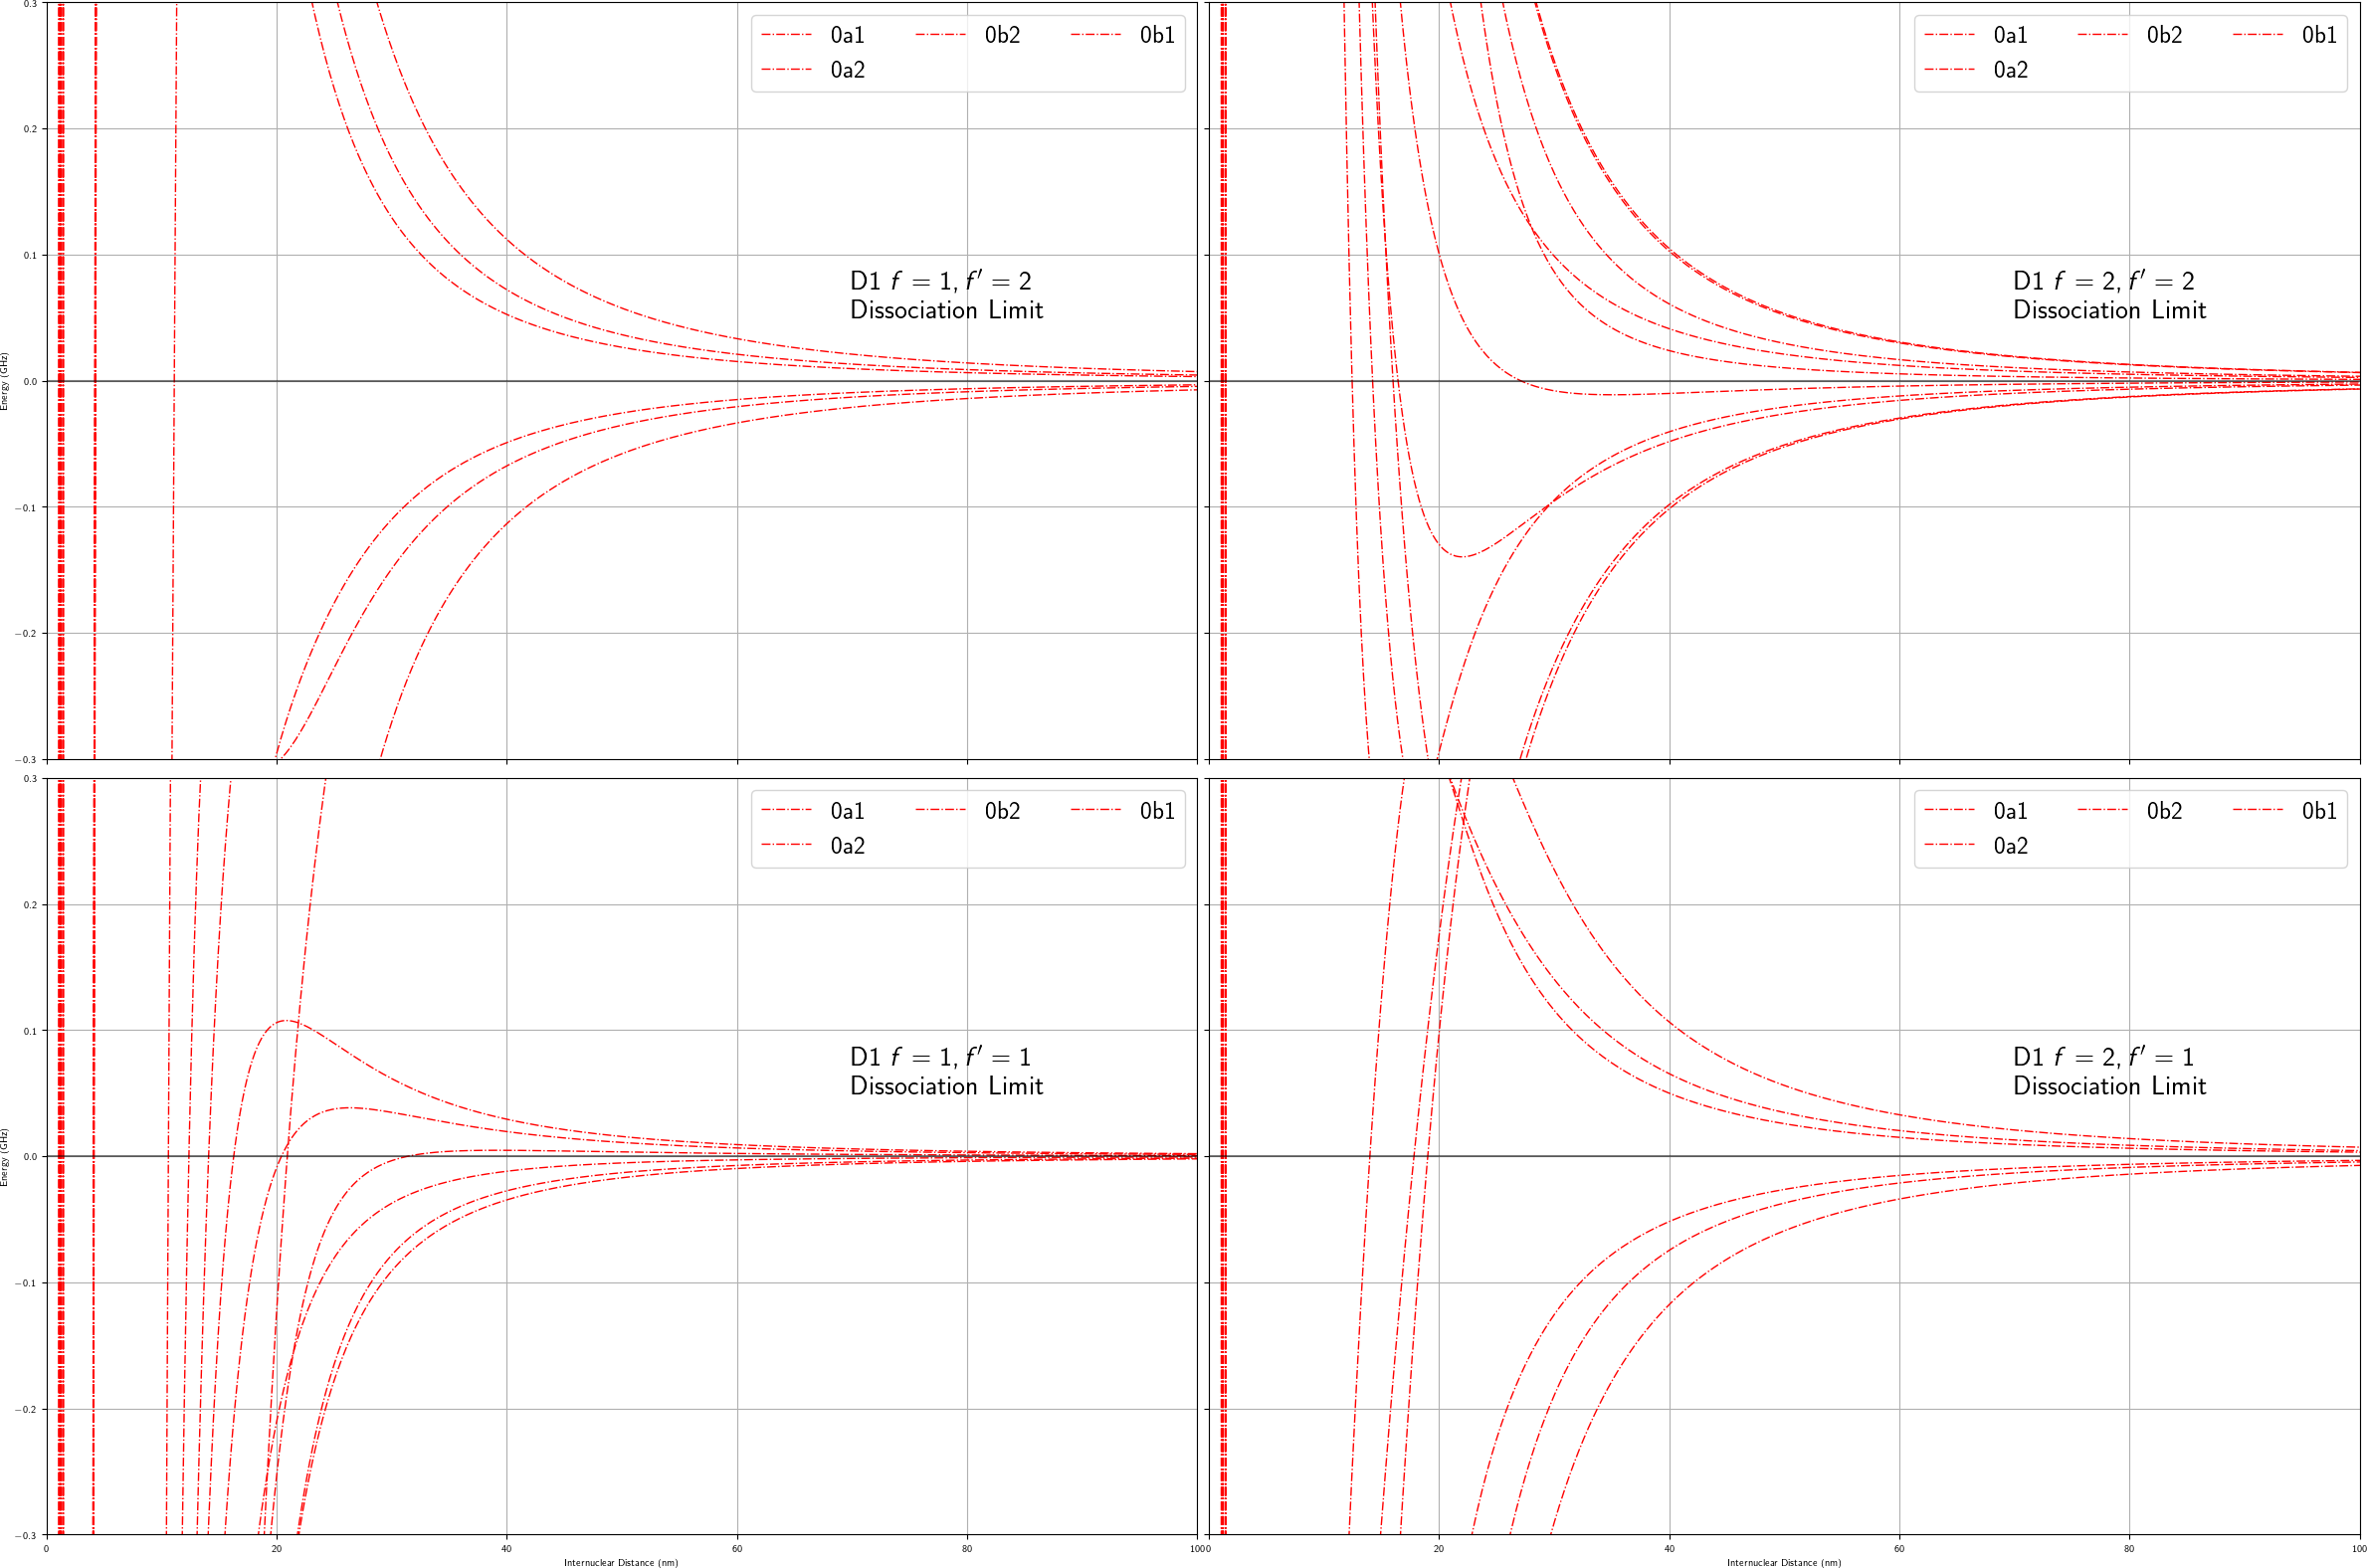
\includegraphics[width=\linewidth]{Symmetrized_Hyperfine_Splitting_D1_Zoom.png}
  \caption{Zoomed in on the D1 Line.}
  \label{fig:boat1}
\end{figure}
\begin{figure}
  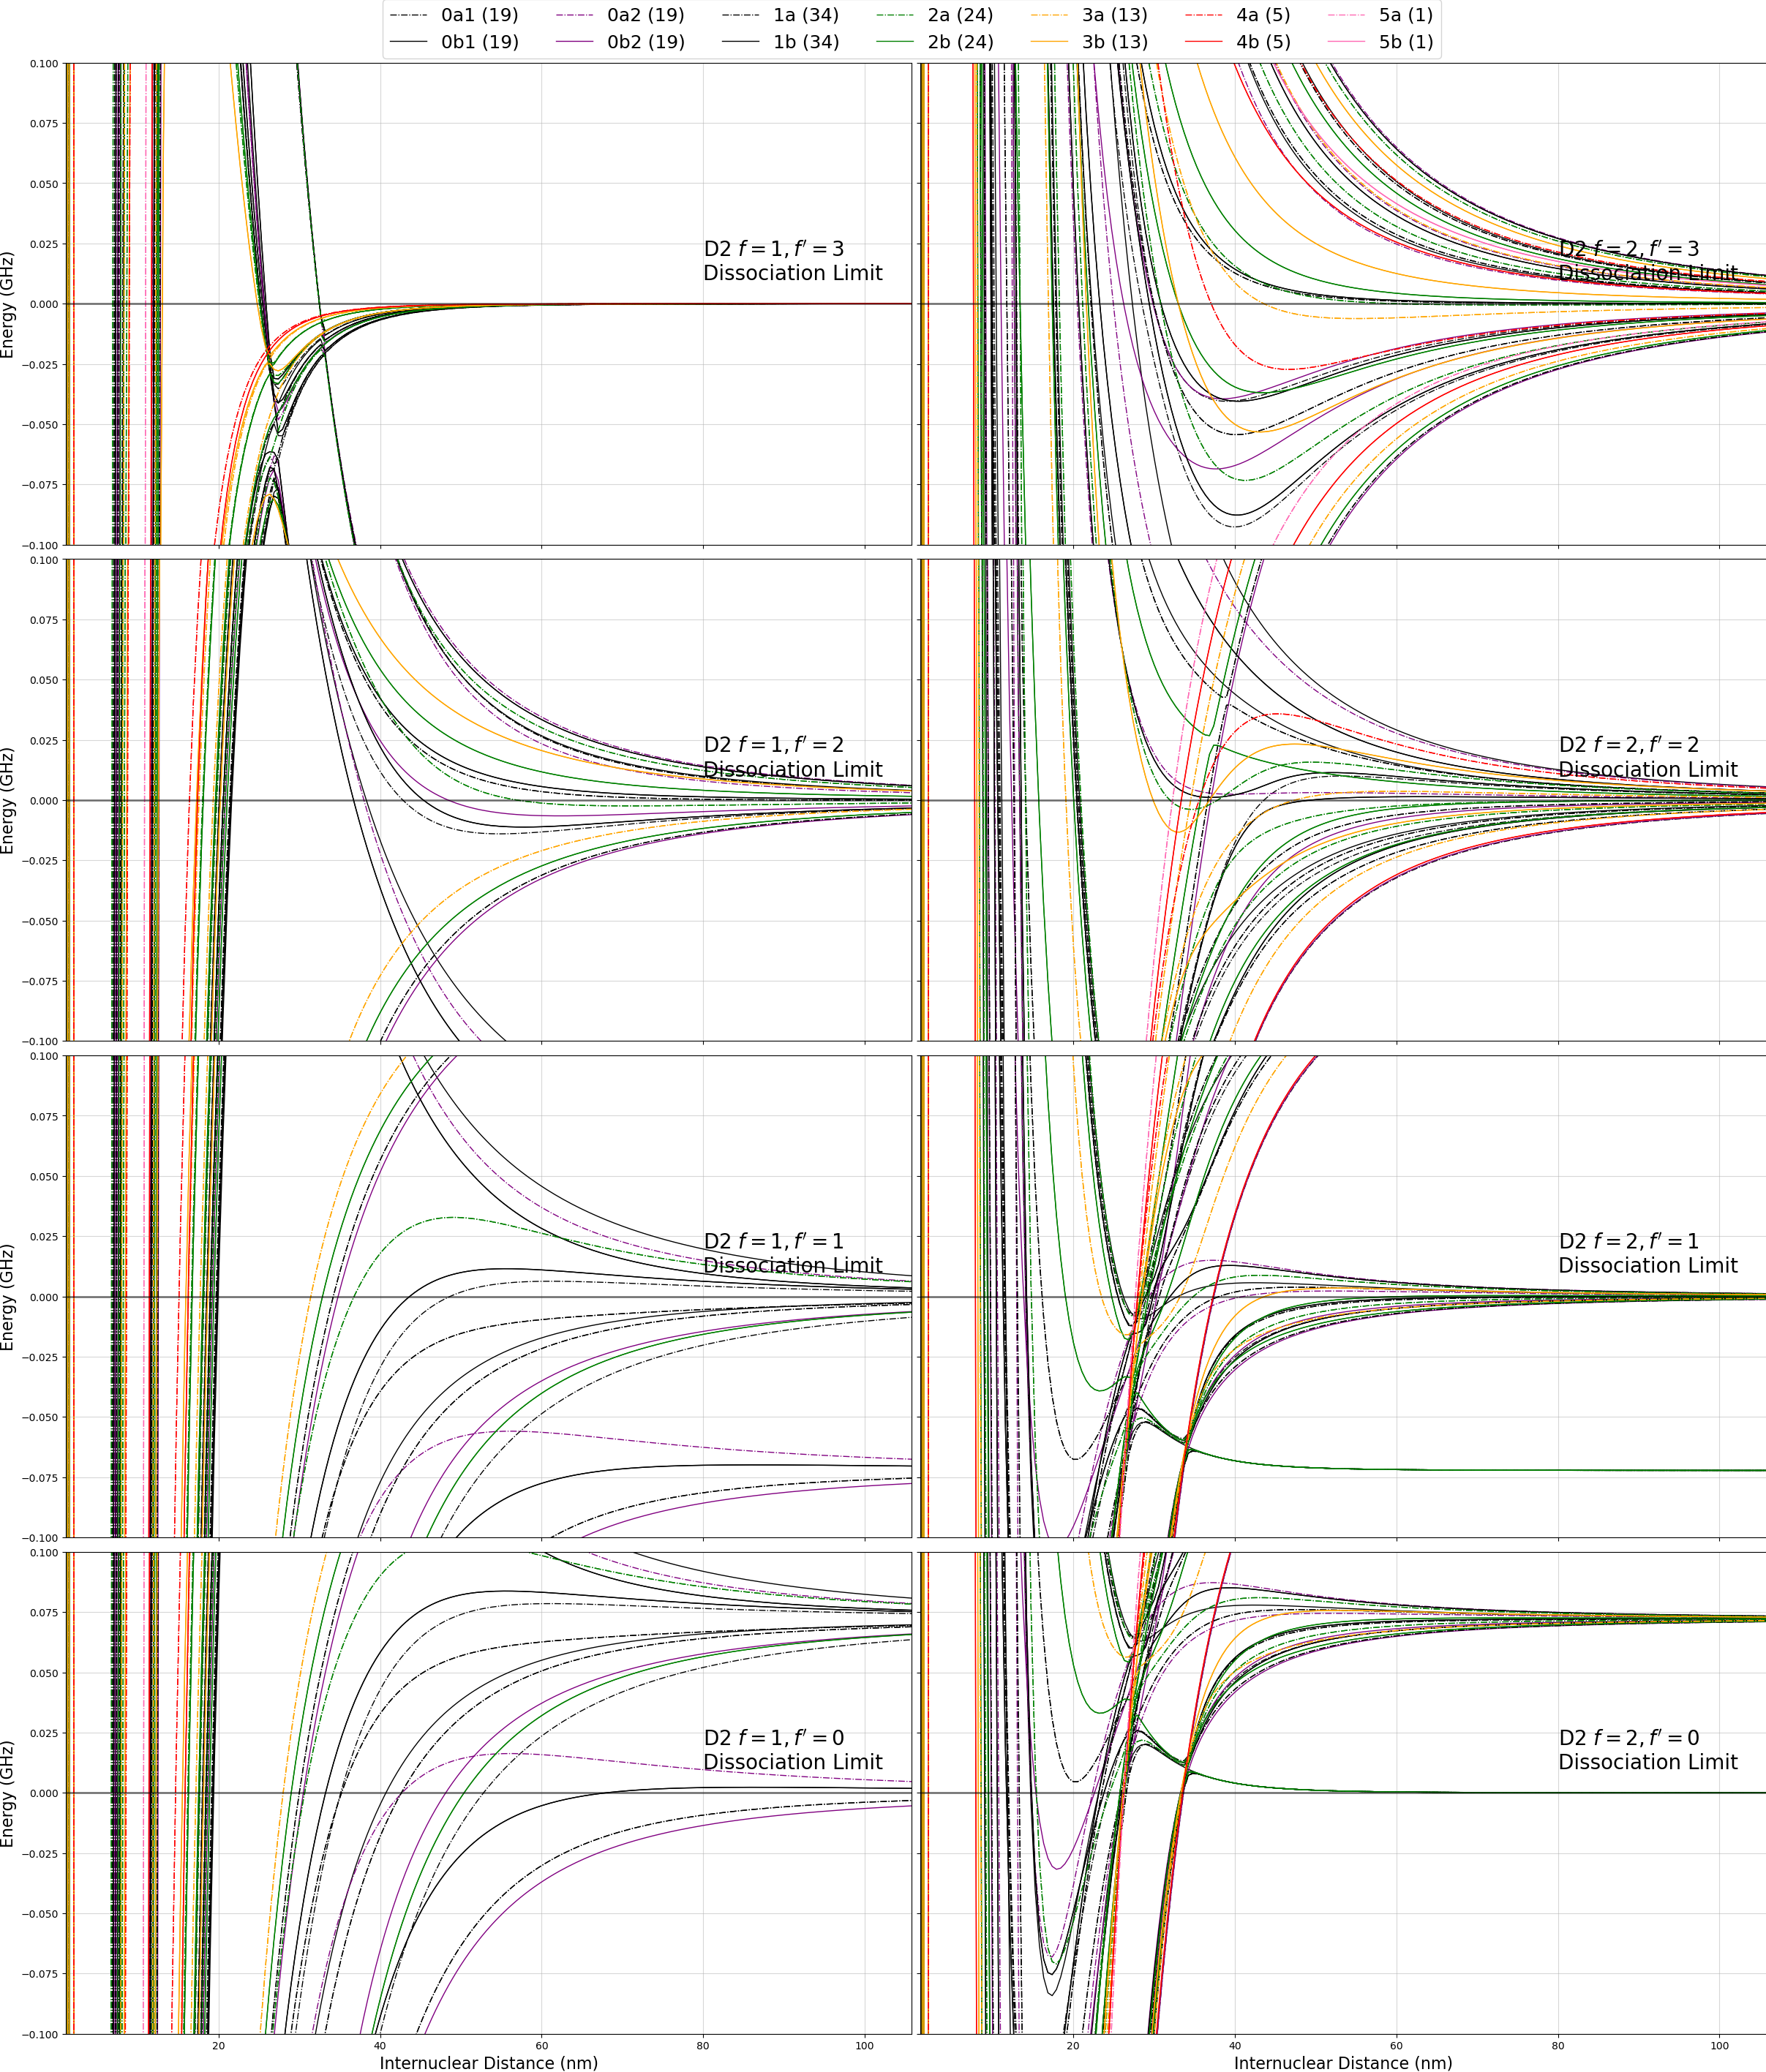
\includegraphics[width=\linewidth]{Symmetrized_Hyperfine_Splitting_D2_Zoom.png}
  \caption{Zoomed in on the D2 Line.}
  \label{fig:boat1}
\end{figure}


\section{Selection Rules}
Currently most of my thoughts on selection rules are coming from \cite{herzberg_spectra_1939}. It seems most likely that the obvious extensions of selection rules hold in the case of hyperfine interactions holding without rotation. That is: $\phi'=\phi+\{0,\pm 1\}$, $\mathbb{i}\pm\leftrightarrow\mathbb{i}\mp$, and $\sigma_v\pm\leftrightarrow\sigma_v\pm$ for states that have well-defined $\sigma_v$. 

\section{Rotation}

Loading experiments are in a unique regime where rotational energy is small compared to all other energy scales. In many molecular experiments, the rotational energy is significant even compared to the fine structure energy scale. The rotational kinetic energy of a rigid rotor is given by $\hbar^2 \ell (\ell+1)/(m_{Rb^{87}}R^2)$ where $R$ is the internuclear distance. Fundamentally, since the loading occurs during sub-doppler cooling, the values this rotational kinetic energy takes are on the order of a couple MHz, and are naturally far below the linewidth of the molecular states involved, and as well much smaller than the hyperfine structure, which is tens to hundreds of MHz large in Rubidium. In general, the coriolis force will mix states of good hyperfine symmetry, but in this region this mixing is small and so states should maintain . This limits the maximum values of $\ell$ available at a given distance. More importantly, the collisions happen at relatively large distance scales, where $R$ is on the order of 10s of nm. Using this info, we can estimate the rotational energy splittings at a given distance as well. The result is displayed in the figure below. It's easy to see that at the distance and energy scales relevant for collisions, the rotational splittings are all well sub-linewidth. As such, they are not resolvable and only contribute to a small extra broadening of the states. We have determined that rotation does not mix states significantly, and rotational levels are not resolvable, therefore we can ignore rotation.\cite{hornkohl_parity_2017}

I think the part of this argument that I'm least convinced of is that the energies are necessarily low, since it's not literally the rotational energy which appears in the hamiltonian, but I think the actual elements should be on this order. 

\begin{figure}
  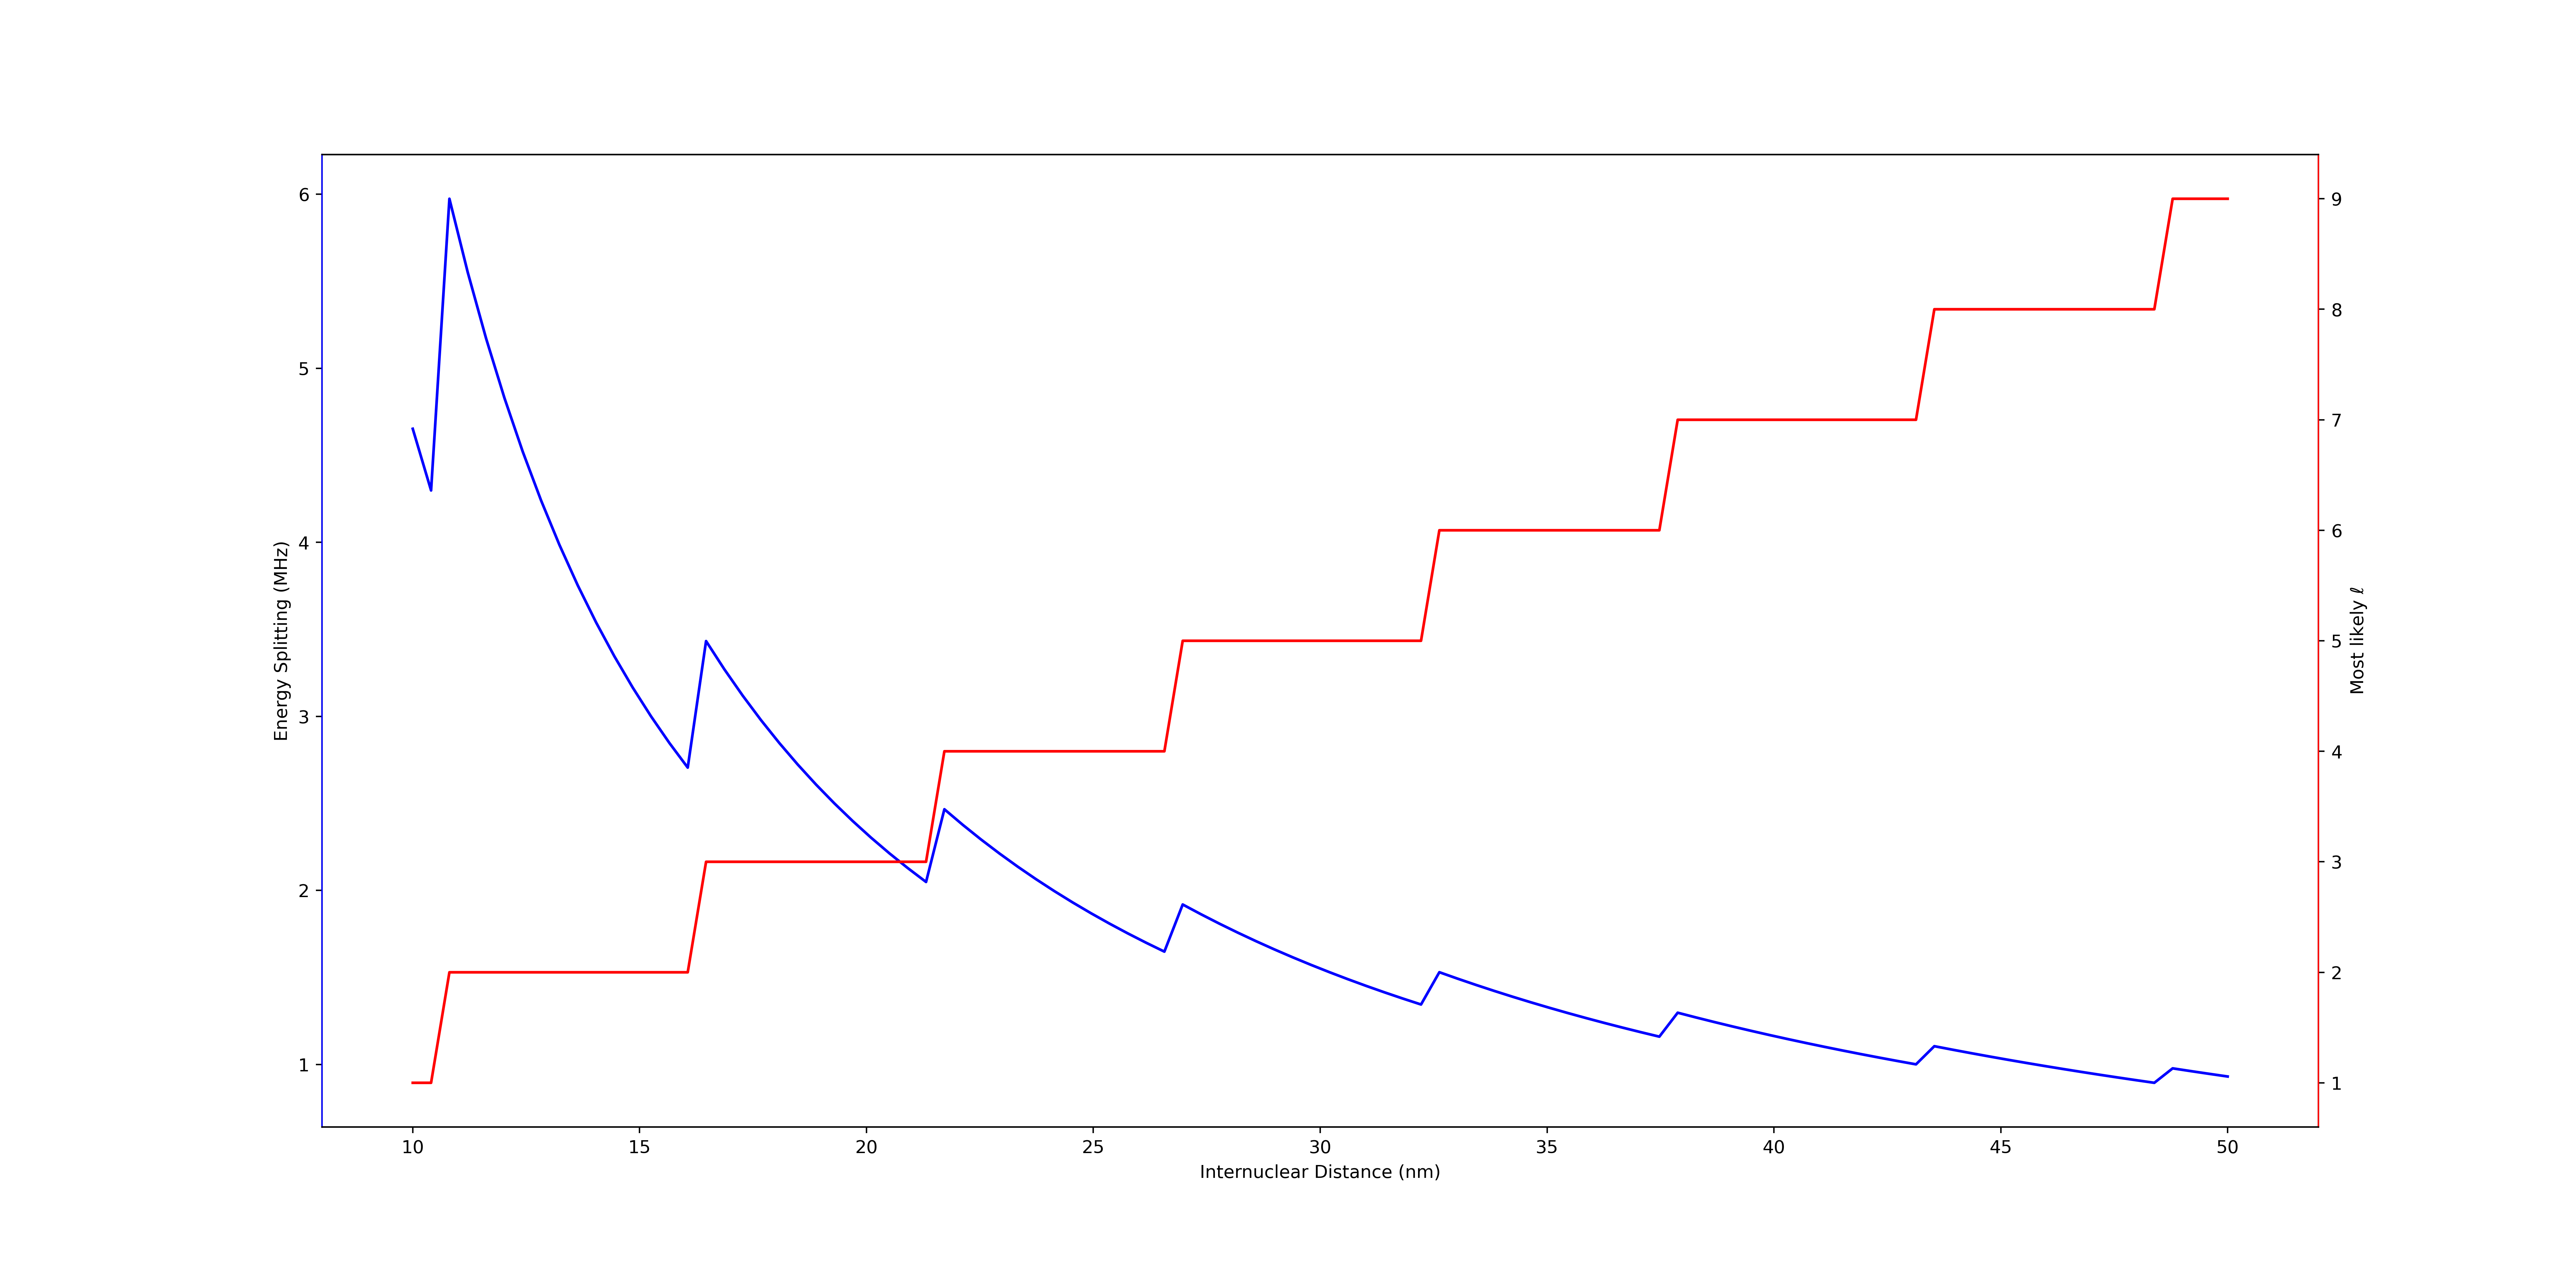
\includegraphics[width=\linewidth]{Rotational_Energy_Separation.png}
  \caption{Rotational Energy Separation Figure.}
  \label{fig:boat1}
\end{figure}

\subsection{Wigner D Functions}

In this section I'm going to try to discuss / better understand the Wigner D functions which appear importantly in rotational calculations for molecules like this. The Wigner D functions are very well known and commonly used, but for some reason I've had trouble finding an introduction to them that is to my tastes, so I'm going to try to make this elementary and instructive. This might be partially because we are entering chemistry grounds, and perhaps chemists are on average less interested in understanding how the functions are derived from first principles. I have two books specifically on quantum angular momentum which have sections on wigner functions: \cite{edmonds_angular_1960} chapter 4 and \cite{varshalovich_quantum_1988} chapter 4. I think that \cite{edmonds_angular_1960} chapter 4 probably has the better intuitive discussion of the functions, and much better than I've seen online.

It should perhaps not be surprising, but analyzing rotations in quantum mechanics benefits from a firm foundation of rotations in classical mechanics, and in particular with the Euler angles.
As such, readers may wish to consult with their own favorite clasical mechanics textbook to remind them of how the Euler angles are typically defined and what purpose they serve. 
Mostly for my own sake here, I'm going to refer to my own classical mechanics textbook from undergraduate studies, \cite{taylor_classical_2005}, which nicely treats (and only treats) the case of the symmetric top.

The euler angles serve to completely and uniquely specify the orientation of a three-dimensional object, and it's body-fixed principle axes which may not be constant in time, with respect to a constant space-fixed axis. Conventions differ, but here I will define the Euler angles as $\alpha, \beta, \text{and} \gamma$. The principle axes of a given body is then found by rotating the space-fixed frame (SFF) first by $\alpha$ about the space-fixed z-axis creating new set of axes (SFF'), then by $\beta$ about the y-axis of the SFF' coordinates creating the SFF'' axes, and then by $\gamma$ about the z-axis of the SFF'' axis. Note that to keep the angles unique, we restrict the angles as such: $0<\alpha<2\pi, 0<\beta<\pi,$ and $0<\gamma<2\pi$. The axes after these three rotations is the principle axis of the rotated body. When the body is rotating, these angles are changing with time. This three-fold rotation operation is typically given by a rotation operator $D\{\alpha,\beta,\gamma\}$. Alternatively, we can represent this operator as

$$
D\{\alpha,\beta,\gamma\}\vec{r}=D\{0,0,\gamma\}D\{0,\beta,0\}D\{\alpha,0,0\}\vec{r}=
\begin{bmatrix}
\cos\{\gamma\} & \sin\{\gamma\} & 0 \\
-\sin\{\gamma\} & \cos\{\gamma\} & 0 \\
0 & 0 & 1
\end{bmatrix}
\begin{bmatrix}
\cos\{\beta\} & 0 & -\sin\{\beta\} \\
0 & 1 & 0 \\
\sin\{\beta\} & 0 & \cos\{\beta\}
\end{bmatrix}
\begin{bmatrix}
\cos\{\alpha\} & \sin\{\alpha\} & 0 \\
-\sin\{\alpha\} & \cos\{\alpha\} & 0 \\
0 & 0 & 1
\end{bmatrix}
\begin{bmatrix}
x\\
y\\
z
\end{bmatrix}
$$

It is important to realize that although $D\{\alpha\beta\gamma\}$ is a function of three angles, it determines all of the important information of the body for it's rigid rotation, and is therefore acts as a sort of proxy for the rotational wavefunction for rigid bodies. As such it is often said that the Wigner functions are the wavefunctions of the symmetric top. 

It should be familiar territory that angular momentum operators appear in the generators of infinitesimal rotations. It is perhaps newer, but hopefully intitive, that the transformations of angular momentum eigenstates $|\ell, m_\ell\rangle$ under finite rotations can be used in a general way to represent finite rotations. In particular, one can reasonably ask what the effect of rotating angular momentum states is, generally represented as

$$
\langle J,M' |D\{\alpha\beta\gamma\} | J, M \rangle \equiv D^J_{MM'}
$$

$D\{\alpha,\beta,\gamma\}$ is an operator-valued function of $\alpha,\beta$ and $\gamma$. $D^J_{MM'}$ is a scalar-valued function, which is an eigenvalue of $J_z$ and $J'_z$ with eigenvalues $\hbar M$ and $\hbar M'$ respectively (easily verifiable given the definition). It is worth noting that the matrix element between states of different total angular momentum $J$ are always zero and hence it is not worth including a second $J'$ variable (rotating a state can change it's projections, but not it's total angular momentum). Secondly, for most purposes here the coordinates $\alpha,\beta,\gamma$ are not important and are omitted (similar to the omittion of $x,y,z$ when specifying the spatial part of the wavefunction).

[Not sure if keeping this]
It is a straight-forward exercise to show that the kinetic energy of the rotating body whose orientation is determined by the three euler angles is given by

$$
T=\frac{1}{2}I_1\Big(\dot{\alpha}^2 \sin^2\{\beta\}+\dot{\beta}^2\Big)
+\frac{1}{2}I_3(\dot{\gamma}+\dot{\alpha}\cos{\beta})^2
$$

We convert this to the quantum kinetic energy operator by first expressing it in terms of generalized momenta $p_\alpha=\partial T/\partial \dot{\alpha}$:

$$
T = \frac{p_\beta^2}{2I_1} + \Big(\frac{\cos^2\{\beta\}}{2I_1 \sin^2\{\beta\}}+\frac{1}{2I_3}\Big)p_\gamma^2+\frac{1}{2I_1 \sin^2\{\beta\}}p_\alpha^2-\frac{2\cos\{\beta\}}{2I_1 \sin^2\{\beta\}}p_\alpha p_\gamma
$$

A "symmetric top" is a 3-dimensional body which has two identical moments of inertia, and in general a non-zero third moment of inertia (like a top, or a dradel). Such systems have cylindrical symmetry, like a homonuclear molecule, which is why this is relevant. As shown by 

% %%%%%%%%%%%%%%%%%%%%%%%%%%%%%%%%%%%%%%%%%%%%%%%%%%%%%%%%%%%%
% %%%%%%%%%%%%%%%%%%%%%%%%%%%%%%%%%%%%%%%%%%%%%%%%%%%%%%%%%%%%
\section{Rotation}
% %%%%%%%%%%%%%%%%%%%%%%%%%%%%%%%%%%%%%%%%%%%%%%%%%%%%%%%%%%%%
% %%%%%%%%%%%%%%%%%%%%%%%%%%%%%%%%%%%%%%%%%%%%%%%%%%%%%%%%%%%%

In general adding rotation to the problem complicates matters greatly. The Hamiltonian here is

\begin{equation}
H_R = \frac{\hat{N}^2}{2\mu R^2}
\end{equation}

$H_R$ doesn't commute with either $H_{BO}$ or $H_{FS}$, so at this point we have three hamiltonians in our main total Hamiltonian. Depending on $R$ and the rotational state, any of these hamiltonians can dominate, and so depending on their relative states different state bases should be used to describe the states. The different cases of which terms are strongest are called Hund's cases in the literature, and there are five of them labeled (a)-(e). $H_{BO}$ is diagonal in case (a) and case (b) states, $H_{FS}$ is diagonal in the case (c) states, and $H_R$ is diagonal in cases (d) and case (e). Therefore, since we have been working in the BO basis for all this work, the challenge of adding this to the hamiltonian to the calculation amounts to finding the transformation matrices which transform states from case (e), where $H_R$ is diagonal and easy to evaluate, to case (a). States in case (e) are described by quantum numbers $J, j, \ell, j_a, $ and $j_b$, therefore the matrix elements we need to calculate are $\langle J, j, \ell, j_a, j_b|J, L\Lambda\sigma S \Sigma\rangle$.

Depending on how strong the rotational couplings are compared to the Born-Oppenheimer interactions and the , some old quantum numbers are no longer good quantum numbers. The BO potentials are derived in case (a/b) (it's agnostic as to which), while the fine-structure potentials use the case (c) basis. 
In the case that rotation is very strong, one goes to case (d) or case (e). In basis E the good quantum numbers are $|J M_J c \Lambda S \Sigma \mathcal{P} \rangle $ where $\mathcal{P}$ describes the total parity of the state, and where $M_J$ is the projection of J on the relevtant rotational axis, \emph{not} the internuclear axis. 
We need to rotate this basis into the basis using projections along the internuclear axis. In general we do this with the \emph{Wigner D-Matrices} represented by the matrix elements $D^J_{M_J,\Omega}=\langle J,M_J|\mathcal{R}\{\alpha,\beta\gamma\}|J, \Omega\rangle$ where $\mathcal{R}\{\alpha,\beta\gamma\}$ are standard 3D rotation matrices with euler angles $\alpha, \beta,$ and $\gamma$. The original reference for this derivation is \cite{singer_theory_1983}, although Paul's notes explain the matter more clearly in my opinion. 
As usual, only the absolute value of the projection is expected to matter, so we will have to include the appropriatly superposition of the two $\Omega$ states. 
Therefore, we expect to be able to write the original basis in the form $|J M_J; L \Lambda L_a L_b; S \Sigma  S_1 S_2; \mathcal{P} \rangle=N(D^{J*}_{M_J\Omega}|L \Lambda L_1 L_2; S \Sigma S_1 S_2\rangle+pD^{J*}_{M_J-\Omega}|L -\Lambda L_1 L_2; S -\Sigma S_1 S_2\rangle)$. One can think about the symmetrization and normalization carefully and come to the conclusion that this must be
\begin{equation}
\begin{split}
|J M_J; L \Lambda L_a L_b; S \Sigma  S_1 S_2; \mathcal{P} \rangle=\\
\frac{1}{\sqrt{2-\delta_{\Lambda 0}\delta_{\Sigma 0}}}\sqrt{\frac{2J+1}{8\pi^3}}\bigg[&D^{J*}_{M_J\Omega}\{\alpha \beta \gamma\}|L \Lambda L_a L_b; S \Sigma S_a S_b\rangle\\
&+\mathcal{P}(-1)^{l_a+l_b+J-S}D^{J*}_{M_J-\Omega}\{\alpha \beta \gamma\}|L, -\Lambda L_a L_b; S, -\Sigma S_a S_b\rangle\bigg]
\end{split}
\end{equation}

We need to represent the $|j\Omega j_a j_b\rangle$ state in terms of the single particle states:
\begin{equation}
|L \Lambda L_1 L_2; S \Sigma S_1 S_2\rangle = \sum_{j, j_a, j_b} |j\Omega j_a j_b\rangle\langle j\Omega j_a j_b | L_a L_b \Lambda_a \Lambda_b; S\Sigma S_a S_b\rangle
\end{equation}

So we need to calculate these matrix elements between the states which are just going to end up giving us a ton of clebsch gordon coefficients: 
\begin{align}
&\langle j\Omega j_a j_b | L_a L_b \Lambda_a \Lambda_b; S\Sigma S_a S_b\rangle \\
= &\Bigg(\sum_{\Omega_a \Omega_b} C_{j_a j_b \Omega_a \Omega_b}^{j \Omega} \langle j_a j_b \Omega_a \Omega_b |\Bigg)|L_a L_b \Lambda_a \Lambda_b\rangle \Bigg(\sum_{\Sigma_a\Sigma_b} C_{S_a S_b \Sigma_a \Sigma_b}^{S \Sigma}| S_a S_b \Sigma_a \Sigma_b\rangle\Bigg)\\
=&\Bigg(\sum_{\Omega_a \Omega_b}C_{j_a j_b \Omega_a \Omega_b}^{j \Omega}\Big(\sum_{\Lambda_a\Sigma_a} C_{L_a S_a \Lambda_a \Sigma_a}^{j_a \Omega_a}\langle L_a S_a \Lambda_a \Sigma_a |\Big)\Big(\sum_{\Sigma_b\Lambda_b} C_{L_b S_b \Lambda_b \Sigma_b}^{j_b \Omega_b}\langle L_b S_b \Lambda_b \Sigma_b |\Big)\Bigg)\\
&\times|L_a L_b \Lambda_a \Lambda_b\rangle\Bigg(\sum_{\Sigma_a\Sigma_b} C_{S_a S_b \Sigma_a \Sigma_b}^{S \Sigma} | S_a S_b \Sigma_a \Sigma_b\rangle\Bigg)\\
=&\sum_{\Sigma_a \Sigma_b \Omega_a \Omega_b} 
C_{j_a j_b \Omega_a \Omega_b}^{j \Omega} 
C_{L_a S_a \Lambda_a \Sigma_a}^{j_a \Omega_a}
C_{L_b S_b \Lambda_b \Sigma_b}^{j_b \Omega_b} 
C_{S_a S_b \Sigma_a \Sigma_b}^{S \Sigma}\\
=&\sum_{L} \sqrt{\breve{S}\breve{j_a}\breve{j_b}\breve{L}} 
C_{L_a L_b \Lambda_a \Lambda_b}^{L \Lambda}
C_{L S \Lambda \Sigma}^{j \Omega}
\begin{Bmatrix}
L_a & S_a & j_a\\
L_b & S_b & j_b\\
L & S & j
\end{Bmatrix}\\
=&\sqrt{\breve{S}\breve{j_a}\breve{j_b}\breve{L}} 
C_{L S \Lambda \Sigma}^{j \Omega}
\begin{Bmatrix}
L_a & S_a & j_a\\
L_b & S_b & j_b\\
L & S & j
\end{Bmatrix}
\end{align}

(should redo to match the 9j definition) Here we have $\breve{x}=2x+1$ where $x$ is any angular momentum quantum number. We can see here that we have to be careful with the signs of the projections, as these will carry through to the clebsch gordon coefficient.  The term in curly brackets is known as the Wigner 9-j symbol - it evaluates to a constant. Where in the last step I used the fact that we know for atoms of interest for us there is only one value of L, specifically $L=L_b=1$ and $L_a=0$ to remove the superfluous clebsch gordon coefficient and sum over $L$. We need to rotate the single particle states. They can be rotated through the following relation:
\begin{equation}
|j\Omega j_a j_b\rangle = \sum_m |j m j_a j_b\rangle D^j_{m \Omega}\{\alpha\beta\gamma\}
\end{equation}

Therefore, equation 15 becomes...
\begin{equation}
\begin{split}
&|J M_J; L \Lambda L_a L_b; S \Sigma  S_1 S_2; \mathcal{P} \rangle
\\
=&\frac{1}{\sqrt{2-\delta_{\Lambda 0}\delta_{\Sigma 0}}}
\sqrt{\frac{2J+1}{8\pi^3}}
\sum_{j, j_a, j_b} 
\bigg[D^{J*}_{M_J\Omega}
|j\Omega j_a j_b\rangle\langle j\Omega j_a j_b | L_a L_b \Lambda_a \Lambda_b; S\Sigma S_a S_b\rangle
\\
&+\mathcal{P}(-1)^{l_a+l_b+J-S}D^{J*}_{M_J-\Omega}
|j,-\Omega j_a j_b\rangle\langle j,-\Omega j_a j_b | L_a L_b \Lambda_a \Lambda_b; S,-\Sigma S_a S_b\rangle
\bigg]
\\
=&\frac{1}{\sqrt{2-\delta_{\Lambda 0}\delta_{\Sigma 0}}}
\sqrt{\frac{2J+1}{8\pi^3}}
\sum_{j, m_j, j_a, j_b} \bigg[
C_{L S \Lambda \Sigma}^{j \Omega}
D^{J*}_{M_J\Omega}D^j_{m \Omega}
|j m j_a j_b\rangle
\\
&+
C_{L,-\Lambda S,-\Sigma}^{j,-\Omega}
\mathcal{P}(-1)^{l_a+l_b+J-S}D^{J*}_{M_J-\Omega}
D^j_{m,-\Omega}|j m j_a j_b\rangle \bigg]
\sqrt{\breve{S}\breve{j_a}\breve{j_b}\breve{L}}
\begin{Bmatrix}
L_a & S_a & j_a\\
L_b & S_b & j_b\\
L & S & j
\end{Bmatrix}
\\
=&\frac{1}{\sqrt{2-\delta_{\Lambda 0}\delta_{\Sigma 0}}}
\sqrt{\frac{2J+1}{8\pi^3}}
\sum_{j, m_j, j_a, j_b} \bigg[
D^{J*}_{M_J\Omega}D^j_{m \Omega}
|j m j_a j_b\rangle
\\
&+
\mathcal{P}(-1)^{l_a+l_b+L-j+J}D^{J*}_{M_J-\Omega}
D^j_{m,-\Omega}|j m j_a j_b\rangle \bigg]
C_{L\Lambda S\Sigma}^{j\Omega}\sqrt{\breve{S}\breve{j_a}\breve{j_b}\breve{L}}
\begin{Bmatrix}
L_a & S_a & j_a\\
L_b & S_b & j_b\\
L & S & j
\end{Bmatrix}
\end{split}
\end{equation}

From \cite{edmonds_angular_1960}  eq. 4.1.25:

\begin{equation}
\begin{split}
D^{\ell}_{\mu 0}\{\alpha\beta\gamma\} = (-1)^\mu \sqrt{\frac{4\pi}{2\ell+1}}Y_{\ell,\mu}(\beta,\alpha)\\
D^{\ell}_{0\mu}\{\alpha\beta\gamma\} = \sqrt{\frac{4\pi}{2\ell+1}}Y_{\ell,\mu}(\beta,\gamma)
\end{split}
\end{equation}

There are a couple important relations for the Wigner D matrix here:

\begin{equation}
\begin{split}
\sqrt{\frac{4\pi}{2\ell+1}}Y_{\ell \mu}\{\beta, \alpha\}=\sqrt{\frac{4\pi}{2\ell+1}}|\ell\mu\rangle
=D^{\ell *}_{\mu 0} \{\alpha \beta \gamma\}
=(-1)^{\mu}D^{\ell}_{-\mu 0} \{\alpha \beta \gamma\}
\\
D^{J*}_{M_J \Omega}\{\alpha,\beta,\gamma\} 
=(-1)^{M_J-\Omega} D_{-M_J,-\Omega}^J\{\alpha,\beta,\gamma\}
\\
D_{-M_j,-\Omega}^{J}
D_{m_j \Omega}^{j}
= \sum_{\ell=|j-j'|}^{j+j'}
C_{J,-M_J j m_j}^{\ell, -\mu}
C_{J,-\Omega j \Omega}^{\ell 0}
D^{\ell}_{-\mu,0}
\end{split}
\end{equation}

We can use these on equation 25. Note that since $\hat{J}=\hat{j}+\hat{N}$, we have $M_J-m_j=\mu$. Therefore:

\begin{equation}
\begin{split}
&|J M_J; L \Lambda L_a L_b; S \Sigma  S_1 S_2; \mathcal{P} \rangle
\\
=&\frac{1}{\sqrt{2-\delta_{\Lambda 0}\delta_{\Sigma 0}}}
\sqrt{\frac{2J+1}{8\pi^3}}
\sum_{j, m_j, j_a, j_b} \bigg[
(-1)^{M_J-\Omega} D_{-M_J,-\Omega}^J
D^j_{m \Omega}
|j m j_a j_b\rangle
\\
&+
\mathcal{P}(-1)^{l_a+l_b+L-j+J}
(-1)^{M_J+\Omega} D_{-M_J\Omega}^J
D^j_{m,-\Omega}|j m j_a j_b\rangle \bigg]
C_{L\Lambda S\Sigma}^{j\Omega}\sqrt{\breve{S}\breve{j_a}\breve{j_b}\breve{L}}
\begin{Bmatrix}
L_a & S_a & j_a\\
L_b & S_b & j_b\\
L & S & j
\end{Bmatrix}
\\
=&\frac{1}{\sqrt{2-\delta_{\Lambda 0}\delta_{\Sigma 0}}}
\sqrt{\frac{2J+1}{8\pi^3}}
\sum_{j, m_j, j_a, j_b,\ell} \bigg[
(-1)^{M_J-\Omega} 
C_{J,-M_J j m_j}^{\ell, -\mu}
C_{J,-\Omega j \Omega}^{\ell 0}
D^{\ell}_{-\mu,0}
|j m j_a j_b\rangle
\\
&+
\mathcal{P}(-1)^{l_a+l_b+L-j+J}
(-1)^{M_J+\Omega} 
C_{J,-M_J j m_j}^{\ell, -\mu}
C_{J\Omega j,-\Omega}^{\ell 0}
D^{\ell}_{-\mu,0}
|j m j_a j_b\rangle \bigg]
C_{L\Lambda S\Sigma}^{j\Omega}\sqrt{\breve{S}\breve{j_a}\breve{j_b}\breve{L}}
\begin{Bmatrix}
L_a & S_a & j_a\\
L_b & S_b & j_b\\
L & S & j
\end{Bmatrix}
\\
=&\frac{1}{\sqrt{2-\delta_{\Lambda 0}\delta_{\Sigma 0}}}
\frac{1}{2\pi}
\sum_{j, m_j, j_a, j_b} 
\sum_{\ell=|j-j'|}^{j+j'} 
(-1)^{-\mu+M_J-\Omega}
\bigg[
C_{J,-\Omega, j \Omega}^{\ell 0}
\\
&+\mathcal{P}(-1)^{l_a+l_b+L+J-j+2\Omega}
C_{J\Omega j,-\Omega}^{\ell 0}
\bigg]
C_{J,-M_J j m_j}^{\ell, -\mu}|\ell\mu\rangle |j m j_a j_b\rangle
\sqrt{\breve{S}\breve{j_a}\breve{j_b}\breve{L}} 
C_{L \Lambda S \Sigma}^{j \Omega}
\begin{Bmatrix}
L_a & S_a & j_a\\
L_b & S_b & j_b\\
L & S & j
\end{Bmatrix}
\end{split}
\end{equation}

Note that there are some very funny clebsch gordon coefficients here that aren't quite what I want. I want to go from $|\ell\mu jm_j\rangle\rightarrow|J M_J \ell j\rangle$, so I need clebsch gordon coefficients of the form $C_{\ell \mu j m_j}^{J M_J}$, not the ones I have here. These are related though, and we need two other clebsch gordon symmetry relations:

\begin{equation}
\begin{split}
C_{\ell \mu j m_j}^{J M_J} = \langle\ell \mu j m_j |J M_J \rangle = (-1)^{j+m_j}\sqrt{\frac{\breve{J}}{\breve{\ell}}}\langle J, -M_J j m_j |\ell, -\mu \rangle\\
C_{J\Omega j,-\Omega}^{\ell 0} = (-1)^{J+j-\ell}C_{J,-\Omega j\Omega}^{\ell 0}\\
C_{J\Omega j,-\Omega}^{\ell 0} = (-1)^{J+j-\ell}C_{j,-\Omega J\Omega}^{\ell 0}\\
\end{split}
\end{equation}

This looks promising because it corrects the signs, but it looks less promising because of the extra funny factor there. But let's try it for a moment:

\begin{equation}
\begin{split}
&|J M_J; L \Lambda L_a L_b; S \Sigma  S_1 S_2; \mathcal{P} \rangle
\\
=&\frac{1}{\sqrt{2-\delta_{\Lambda 0}\delta_{\Sigma 0}}}
\frac{1}{2\pi}
\sum_{j, m_j, j_a, j_b} 
\sum_{\ell=|j-j'|}^{j+j'} 
(-1)^{j-\mu+M_J+m_j-\Omega}
\bigg[
(-1)^{2j+2J-2\ell}
\\
&+\mathcal{P}(-1)^{l_a+l_b+L+J-j+2\Omega}
(-1)^{j+J-\ell}
\bigg]
C_{j,-\Omega J\Omega}^{\ell 0}
C_{\ell \mu j m_j}^{J M_J}
|\ell\mu\rangle |j m j_a j_b\rangle
\sqrt{\breve{S}\breve{j_a}\breve{j_b}\breve{L}} 
C_{L \Lambda S \Sigma}^{j \Omega}
\begin{Bmatrix}
L_a & S_a & j_a\\
L_b & S_b & j_b\\
L & S & j
\end{Bmatrix}
\\
=&\frac{1}{\sqrt{2-\delta_{\Lambda 0}\delta_{\Sigma 0}}}
\frac{1}{2\pi}
\sum_{j, m_j, j_a, j_b} 
\sum_{\ell=|j-j'|}^{j+j'} 
(-1)^{j-\mu+M_J+m_j-\Omega+2j+2J-2\ell}
\bigg[\\
&1+\mathcal{P}(-1)^{l_a+l_b+L-2j+2\Omega+\ell}
\bigg]
C_{j,-\Omega J\Omega}^{\ell 0}
(-1)^{j+\ell-J}
C_{j m_j\ell \mu}^{J M_J}
|\ell\mu\rangle |j m j_a j_b\rangle
\sqrt{\breve{S}\breve{j_a}\breve{j_b}\breve{L}} 
C_{L \Lambda S \Sigma}^{j \Omega}
\begin{Bmatrix}
L_a & S_a & j_a\\
L_b & S_b & j_b\\
L & S & j
\end{Bmatrix}
\\
=&\frac{1}{\sqrt{2-\delta_{\Lambda 0}\delta_{\Sigma 0}}}
\frac{1}{2\pi}
\sum_{j, m_j, j_a, j_b} 
\sum_{\ell=|j-j'|}^{j+j'} 
(-1)^{-\mu+M_J+m_j-\Omega+J-\ell}
\bigg[\\
&1+\mathcal{P}(-1)^{l_a+l_b+L-2j+2\Omega+\ell}
\bigg]
C_{j,-\Omega J\Omega}^{\ell 0}
C_{j m_j\ell \mu}^{J M_J}
|\ell\mu\rangle |j m j_a j_b\rangle
\sqrt{\breve{S}\breve{j_a}\breve{j_b}\breve{L}} 
C_{L \Lambda S \Sigma}^{j \Omega}
\begin{Bmatrix}
L_a & S_a & j_a\\
L_b & S_b & j_b\\
L & S & j
\end{Bmatrix}\\
=??&\frac{1}{\sqrt{2-\delta_{\Lambda 0}\delta_{\Sigma 0}}}
\frac{1}{2\pi}
\sum_{j, m_j, j_a, j_b} 
\sum_{\ell=|j-j'|}^{j+j'} 
(-1)^{\ell-J-\Omega}
\bigg[\\
&1+\mathcal{P}(-1)^{l_a+l_b+L+\ell}
\bigg]
C_{j,-\Omega J\Omega}^{\ell 0}
C_{j m_j\ell \mu}^{J M_J}
 |j m j_a j_b\rangle|\ell\mu\rangle
\sqrt{\breve{S}\breve{j_a}\breve{j_b}\breve{L}} 
C_{L \Lambda S \Sigma}^{j \Omega} 
\begin{Bmatrix}
L_a & S_a & j_a\\
L_b & S_b & j_b\\
L & S & j
\end{Bmatrix}
\end{split}
\end{equation}

In the last step I assume that J, j, and Omega are integer values such that $(-1)^{2J}=1$ etc. This allows me to remove 2x factors in these phases, and flip signs of these quantum numbers as well as the $m_j$ projection which allowed me to cancel the $\mu, M_J, \text{ and } m_j$ terms in the overall phase. I also can't fully justify needing the flipped clebsch gordon coefficient in the second to last step, although this seems plausible to me if I just screwed up the order of the Wigner D matrices somehow. The order suggested by the text would have put the two matrices sandwhiching a state, so perhaps I screwed up the commutation rules which I don't know at that point and that caused issues. 

\begin{equation}
\begin{split}
&|J M_J; L \Lambda L_a L_b; S \Sigma  S_1 S_2; \mathcal{P} \rangle=
\\
&\frac{1}{\sqrt{2-\delta_{\Lambda 0}\delta_{\Sigma 0}}}
\frac{1}{2\pi}
\sum_{j, m_j, j_a, j_b} 
\sum_{\ell=|j-j'|}^{j+j'} 
(-1)^{\ell-J-\Omega}
\bigg[
1+\mathcal{P}(-1)^{l_a+l_b+L+\ell}
\bigg]
|J M_J j \ell j_a j_b\rangle
\sqrt{\breve{S}\breve{j_a}\breve{j_b}\breve{L}} 
C_{j,-\Omega J\Omega}^{\ell 0}
C_{L \Lambda S \Sigma}^{j \Omega}
\begin{Bmatrix}
L_a & S_a & j_a\\
L_b & S_b & j_b\\
L & S & j
\end{Bmatrix}
\end{split}
\end{equation}

This is extremely close at this point. At this point the only remaining issue is the extra L in the phase in the middle. 

In the end, the conversion between case (a) and case (e) is then given by the following:
\begin{equation}
\langle j \ell j_a j_b | \Lambda S \Sigma p\rangle_J = (-1)^{\ell-\Omega-J} \frac{1+(-1)^{L_b+\ell+p}(1-\delta_{\Lambda,0}\delta_{\Sigma,0})}{\sqrt{2-\delta_{\Lambda,0}\delta_{\Sigma,0}}}\sqrt{\breve{S}\breve{j_a}\breve{j_b}\breve{L}} C_{j,-\Omega J\Omega}^{\ell 0}C_{L\Lambda S\Sigma}^{j\Omega}
\begin{Bmatrix}
L_a & S_a & j_a\\
L_b & S_b & j_b\\
L & S & j
\end{Bmatrix}
\end{equation}

This nasty relation allows you to calculation transformation matrices to convert all the case (e) basis states to case (a) in order to evaluate the hamiltonian for each value of $\ell$ and as a function of R. For the record I'm not sure using the 9j symbol here really makes things simpler, but okay. 

For a given value of J, states can have either positive or negative total parity. It turns out that the results of these calculations result in pairs of closely spaced rotational energy levels which have different pairity, and so each state gets an additional label. States with parities $(-1)^J$ are said to have "e" parity, and states with pairities $-(-1)^J$ are said to have "f" parity. This scheme ensures that each state in the doublet has different such parity, and as well the "e" and "f" are independent of the hunds case basis used. In other words, the matrix elements above do not mix states of different "e/f" parity. This parity label has historically fluctuated and been the source of confusion in the field \cite{hornkohl_parity_2017,brown_labeling_1975}.

In the end, I can use this calculation to calculate the rotational couplings, as shown in figure (2)

\section{Hyperfine Rotation}

The state given by paul is

\begin{equation}
\begin{split}
|F M_F c \Lambda S \Sigma I \iota p\rangle \rightarrow \frac{1}{\sqrt{2-\delta_{\Lambda 0}\delta_{\Sigma 0} \delta_{\iota 0}}} \sum_{\ell f f_a f_b}(-1)^{\ell-\phi-F}|F M_F \ell f c_a f_a c_b f_b\rangle\Big[1+(1-\delta_{\Lambda 0}\delta_{\Sigma 0} \delta_{\iota 0})\Big]
C_{f -\phi F \phi}^{\ell 0} \\
\langle f \phi f_a f_b | \Lambda_a \Lambda_b | c \Lambda \rangle \langle \Lambda_a \Lambda_b| c \Lambda \rangle XXXXX
\end{split}
\end{equation}

There's at least one fairly obvious problem here which is the lack of a phase factor for the $(1-\delta)$ term. The term serves to zero terms that have the wrong parity of some sort here, and it doesn't do that. In the previous rotational papers, the phase of this term was $(-1)^{L_b+\ell +p}$. This term makes no explicit reference to $J$ so I think it should actually be the same here. The paper here might have wanted to be more general than this term, but for my purposes there's no need at the moment. Before I continue, I need to deal with the giant matrix element there. 


There are 6 basic angular momentum and multiple ways to couple them to construct states of total angular momentum $f$. As there are so many angular momentum, it seems probably possible to write this big matrix element in terms of the 15j symbols, but there is vanishingly little resources on such symbols, so the better approach is to use the 9j symbols for the coupling of 4 angular momentum. 

In general, suppose you have 4 angular momentum $j_i, i\in\{1,2,3,4\}$. Then, denote $\hat{j}_{ij}=\hat{j}_i+\hat{j}_j$, and $j_{1234}\equiv j_*$ for brevity. There is a common matrix element to consider between the coupling of these four angular momentum:

\begin{equation}
\langle j_{*} m_{j_{*}} j_{12}j_{34}|j_{*} m_{j_{*}}j_{13}j_{24}\rangle
\equiv\sqrt{\breve{j}_{12}\breve{j}_{34}\breve{j}_{13}\breve{j}_{24}}
\begin{Bmatrix}
j_1 & j_2 & j_{13}\\
j_3 & j_4 & j_{34}\\
j_{13} & j_{24} & j_{*}\\
\end{Bmatrix}
\end{equation} 

In the case here, there are two ways to construct the total electronic angular momentum $j$ (not using general notation here). We have $\hat{j}=\hat{l}_a+\hat{s}_a+\hat{l}_b+\hat{s}_b$, and we can first couple the two orbitatal angular momentums and spins to create states $|jm_j L S l_1 l_2 s_1 s_2 \rangle\equiv|j m_j L S\rangle$, or we can construct the individual electronic angular momentum first and create states $|j m_j j_1 j_2 l_1 s_1 l_2 s_2\rangle\equiv|j m_j j_1 j_2\rangle$. Similarly, we have four angular momentum $j_a, j_b, i_a, $ and $i_b$ to construct states of good $f$ in two critical ways to create two bases: $|f m_f j I\rangle$ or $|f m_f f_a f_b\rangle$. This is going to lead to two wigner 9j symbols. And this is suggestive that we are looking to construct the matrix elements $\langle f m_f f_1 f_2 | f m_f j I\rangle$ and $\langle j m_j j_1 j_2| j m_J L S\rangle$ out of the given matrix element, both of which will reduce to clesch gordon coefficients. From here, it's just basic angular momentum algebra to get to the desired result. 

\begin{equation}
\begin{split}
\langle f \phi f_a f_b |\Lambda_a \Lambda_b S\Sigma I\iota\rangle
\xrightarrow{R\rightarrow\infty}
\langle f \phi f_a f_b |l_a\Lambda_a l_b\Lambda_b S\Sigma I\iota\rangle\\
= \langle f \phi f_a f_b | \Bigg(\sum_{L} C^{L\Lambda}_{l_a \Lambda_a, l_b \Lambda_b} |L \Lambda\rangle\Bigg) | S\Sigma I\iota\rangle\\
= \sum_{L} C^{L\Lambda}_{l_a \Lambda_a, l_b \Lambda_b} \langle f \phi f_a f_b | \Big(\sum_{j}C_{L\Lambda S\Sigma}^{j\Omega} |j\Omega L S\rangle\Big) | I\iota\rangle\\
= \sum_{L, j} C^{L\Lambda}_{l_a \Lambda_a, l_b \Lambda_b} C_{L\Lambda S\Sigma}^{j\Omega} \langle f \phi f_a f_b | \Bigg(\sum_{j_1 j_2} |j\Omega j_1 j_2 \rangle\langle j\Omega j_1 j_2 |j\Omega L S\rangle\Bigg) | I\iota\rangle\\
= \sum_{L, j, j_1 j_2} 
C^{L\Lambda}_{l_a \Lambda_a, l_b \Lambda_b} 
C_{L\Lambda S\Sigma}^{j\Omega} 
\langle f \phi f_a f_b | |j\Omega j_1 j_2 \rangle | I\iota\rangle
\sqrt{\breve{j}_1\breve{j_2}\breve{L}\breve{S}}
\begin{Bmatrix}
l_a & s_a & j_a\\
l_b & s_b & j_b\\
L & S & j
\end{Bmatrix}\\
= \sum_{L, j, j_1 j_2} 
C^{L\Lambda}_{l_a \Lambda_a, l_b \Lambda_b} 
C_{L\Lambda S\Sigma}^{j\Omega} 
\langle f \phi f_a f_b | \Bigg(\sum_{f'} C_{j\Omega I \iota}^{f' \phi} |f' \phi j I\rangle\Bigg)
\sqrt{\breve{j}_1\breve{j_2}\breve{L}\breve{S}}
\begin{Bmatrix}
l_a & s_a & j_a\\
l_b & s_b & j_b\\
L & S & j
\end{Bmatrix}\\
= \sum_{L, j, j_1 j_2} 
C^{L\Lambda}_{l_a \Lambda_a, l_b \Lambda_b} 
C_{L\Lambda S\Sigma}^{j\Omega} 
 C_{j\Omega I \iota}^{f \phi}
\langle f \phi f_a f_b |f \phi j I\rangle
\sqrt{\breve{j}_1\breve{j_2}\breve{L}\breve{S}}
\begin{Bmatrix}
l_a & s_a & j_a\\
l_b & s_b & j_b\\
L & S & j
\end{Bmatrix}\\
= \sum_{L, j, j_1 j_2} 
\bigg(
C^{L\Lambda}_{l_a \Lambda_a, l_b \Lambda_b} 
C_{L\Lambda S\Sigma}^{j\Omega} 
C_{j\Omega I \iota}^{f \phi}
\bigg)
\sqrt{\breve{j}_1\breve{j_2}\breve{f}_1\breve{f_2}
\breve{L}\breve{S}\breve{J}\breve{I}}
\begin{Bmatrix}
l_a & s_a & j_a\\
l_b & s_b & j_b\\
L & S & j
\end{Bmatrix}
\begin{Bmatrix}
j_a & i_a & f_a\\
j_b & i_b & f_b\\
j & I & f
\end{Bmatrix}
\end{split}
\end{equation}


Therefore, I plug in the phase factor discussed above, substitue the giant matrix element, and simplify that the last matrix element above is unity, to get

\begin{equation}
\begin{split}
|F M_F c \Lambda S \Sigma I \iota p\rangle \rightarrow \frac{1}{\sqrt{2-\delta_{\Lambda 0}\delta_{\Sigma 0} \delta_{\iota 0}}} \sum_{\ell f f_a f_b}(-1)^{\ell-\phi-F}
|F M_F \ell f c_a f_a c_b f_b\rangle
\Big[1+(-1)^{L_b+\ell+p}(1-\delta_{\Lambda 0}\delta_{\Sigma 0} \delta_{\iota 0})\Big]
C_{f -\phi F \phi}^{\ell 0} \\
\times\sum_{L, j, j_1 j_2} 
\bigg(
C^{L\Lambda}_{l_a \Lambda_a, l_b \Lambda_b} 
C_{L\Lambda S\Sigma}^{j\Omega} 
C_{j\Omega I \iota}^{f \phi}
\bigg)
\sqrt{\breve{j}_1\breve{j_2}\breve{f}_1\breve{f_2}
\breve{L}\breve{S}\breve{J}\breve{I}}
\begin{Bmatrix}
l_a & s_a & j_a\\
l_b & s_b & j_b\\
L & S & j
\end{Bmatrix}
\begin{Bmatrix}
j_a & i_a & f_a\\
j_b & i_b & f_b\\
j & I & f
\end{Bmatrix}
\end{split}
\end{equation}

And therefore I can calculate the matrix element:

\begin{equation}
\begin{split}
\langle F M_F \ell f c_a f_a c_b f_b |F M_F c \Lambda S \Sigma I \iota p\rangle
\\
= 
(-1)^{\ell-\phi-F}
\frac{\Big[1+(-1)^{L_b+\ell+p}(1-\delta_{\Lambda 0}\delta_{\Sigma 0} \delta_{\iota 0})\Big]}
{\sqrt{2-\delta_{\Lambda 0}\delta_{\Sigma 0} \delta_{\iota 0}}} 
C_{f -\phi F \phi}^{\ell 0} 
\\
\times\sum_{j, j_1 j_2} 
\bigg(
C_{L\Lambda S\Sigma}^{j\Omega} 
C_{j\Omega I \iota}^{f \phi}
\bigg)
\sqrt{\breve{j}_1\breve{j_2}\breve{f}_1\breve{f_2}
\breve{L}\breve{S}\breve{J}\breve{I}}
\begin{Bmatrix}
l_a & s_a & j_a\\
l_b & s_b & j_b\\
L & S & j
\end{Bmatrix}
\begin{Bmatrix}
j_a & i_a & f_a\\
j_b & i_b & f_b\\
j & I & f
\end{Bmatrix}
\end{split}
\end{equation}

I set $l_a=0, l_b=1, L=1, s_a=s_b=1/2,j_a=1/2$ as the unique values for singly excited alkali metals, and $i_a=i_b=3/2$ for rubidium 87.

\begin{equation}
\begin{split}
\langle F M_F \ell f c_a f_a c_b f_b |F M_F c \Lambda S \Sigma I \iota p\rangle
\\
= 
(-1)^{\ell-\phi-F}
\frac{\Big[1+(-1)^{L_b+\ell+p}(1-\delta_{\Lambda 0}\delta_{\Sigma 0} \delta_{\iota 0})\Big]}
{\sqrt{2-\delta_{\Lambda 0}\delta_{\Sigma 0} \delta_{\iota 0}}} 
C_{f -\phi F \phi}^{\ell 0} 
\\
\times\sum_{j, j_2} 
\bigg(
C_{L\Lambda S\Sigma}^{j\Omega} 
C_{j\Omega I \iota}^{f \phi}
\bigg)
\sqrt{2\breve{j_2}\breve{f}_1\breve{f_2}
\breve{L}\breve{S}\breve{J}\breve{I}}
\begin{Bmatrix}
0 & 1/2 & 1/2\\
1 & 1/2 & j_b\\
1 & S & j
\end{Bmatrix}
\begin{Bmatrix}
1/2 & 3/2 & f_a\\
j_b & 3/2 & f_b\\
j & I & f
\end{Bmatrix}
\end{split}
\end{equation}

I'm reasonably confident that this result is correct. I'm a little concerned about the sum over $j$ and $j_b$. I think I may e able to remove the sum over $j_b$ at least since I think that $j_b$ is implcitly known from knowing $f_b$ since the complete state would normally be $|f_b, m_{f_b}, j_b, i_b, s_b, l_b\rangle$. Note that for levels of so-called "e" parity are to have total parity of $(-1)^F$, and levels of "f" parity have total parity $-(-1)^F$.  

Before, the rotational hamiltonian only coupled states of the same J, so in this case, same F. in the fine structure case, we had $j_a=1/2, j_b\in\{1/2,3/2\}$ and therefore $j\in\{0,1,2\}$ and now we have $f_a\in\{1,2\}, f_b\in\{0,1,2,3\}$ and therefore $f\in\{0,1,2,3,4,5\}$. 

Paul reports in an old email conversation that for $F=0,1,2,3,4, $ and $5$ or larger there are $19, 53, 77, 90, 95, $ and $96$ states respectively. I think that these states only have F and p quantum numbers. 

\bibliographystyle{plain} 
\bibliography{Near-Threshold-Molecules}

\end{document}
